\documentclass[output=paper]{langsci/langscibook} 

\author{Ekaterina Vylomova\orcid{0000-0002-4058-5459}\affiliation{The University of Melbourne}  and Nick Haslam\orcid{0000-0002-1913-2340}\affiliation{The University of Melbourne}}

\title{Semantic changes in harm-related concepts in English}

\abstract{The chapter investigates semantic changes in core concepts of psychology, specifically focusing on those related to harm. \citet{haslam2016concept} hypothesized that many psychological concepts associated with harm (i.e., forms of psychological disturbance, threat, and maltreatment) have undergone semantic broadening in the past half-century in association with cultural shifts and social change. The implications of this ``concept creep'' hypothesis have been previously explored by prominent social, political, and legal thinkers \citep{levari2018prevalence, lukianoff2019coddling, pinker2018enlightenment,sunstein2018power}, but its linguistic dimension has received little empirical attention.

Here we apply computational models in order to address the concept creep hypothesis. We start with a description of a typology of semantic shifts and provide a summary of computational methods for automatic detection of the most common changes (broadening, narrowing, hyperbole, and litotes) and utilise those to evaluate core harm-related concepts such as `trauma', `harassment', and `bullying' on a new corpus of psychology literature extending from 1970 to 2017. Our results confirm the initial hypothesis and are in line with earlier studies: most concepts became broader and milder over the last few decades. We then continue with a more detailed study in order to understand how exactly the concepts changed, and to do so employ and evaluate different types of semantic representations. 

Finally, we additionally train the models on a general domain corpus in order to investigate whether the broadening of harm-related concepts also applies to society at large, rather than only to the academic discourse of psychology. Haslam's influential account of concept creep \citep{haslam2016concept} proposes that broadened concepts of harm disseminate from academic language into wider public use. This final analysis enables a direct test of that conjecture, including comparative analysis of the extent and timing of historical semantic changes across the two corpora.}


\begin{document}
\SetupAffiliations{mark style=none}
\maketitle


\section{Introduction}\largerpage
Recent years witnessed significant progress in many downstream tasks in natural language processing (NLP) such as machine translation, part-of-speech tagging, language modelling, and many others.\footnote{See \url{https://nlpprogress.com/} for most recent state-of-the-art models in each task.}
Unlike earlier machine learning models that were often provided with a set of pre-designed features or rules, most recent models inherently ``learn'' them from raw data in the form of dense vectors (embeddings). Training strategies used in the models to learn the embeddings often rely on the distributional semantics hypothesis that states that a word's meaning can be expressed as a distribution over a set of its contexts \citep{firth1957synopsis,harris1954distributional,weaver1955translation}. A significant amount of research works explored what aspects of language are captured in these representations. Although the distributional semantics approach presents certain limitations \citep{bender2020climbing}, it still allows to extract a surprising amount of information about semantic, morphological, and syntactic properties of language \citep{mikolov2013linguistic,vylomova2016take,gladkova2016analogy,belinkov2019analysis,rogers2020primer}.
In addition, representations obtained using this approach capture associations between words and can potentially simulate surveys on free word associations \citep{agirre2009study,antoniak2018evaluating}.
These successes induced a novel direction of interdisciplinary studies -- corpus-centered research -- where embeddings are used as a direct evidence about the language and culture of the authors of a training corpus \citep{antoniak2018evaluating}.
For instance, \citet{hamilton-etal-2016-cultural,hamilton-etal-2016-diachronic} presented one of the earliest diachronic language models and metrics to evaluate semantic shifts as well as 
computational approaches to lexical semantic change detection. Over the last few years, the area has significantly increased and witnessed substantial progress and development \citep{schlechtweg-etal-2020-semeval}.

In this chapter, we apply diachronic language modelling to computationally attest semantic shifts in core concepts of social psychology. In particular, we focus on diachronic change in the meaning of harm-related concepts and test a ``concept creep'' hypothesis proposed in \citet{haslam2016concept}. The hypothesis states that during the past half-century many concepts associated with harm have broadened their meanings in Western societies.
We quantitatively evaluate changes in the five negative concepts: `addiction', `bullying', `harassment', `prejudice', and `trauma'. We attest them on a newly introduced corpus of psychology journal abstracts and a general domain corpus comprising CoCA and CoHA.
In order to test the hypothesis, we first conduct frequency-based analysis and then study the changes in a greater detail by evaluating vector representations learned by epoch-specific models trained on each corpus.


\section{The notion of concept creep}
\citet{haslam2016concept} introduced the idea of ``concept creep'' to describe a general pattern of semantic inflation in several fundamental psychological concepts. The paper presented a series of case studies in which psychological researchers and theorists expanded the sense of harm-related concepts by loosening definitions to include milder instances (``vertical creep'') or by extending definitions to encompass qualitatively new phenomena (``horizontal creep''). 

The two forms of creep can be understood from the perspective of Bloomfield's typology of lexical semantic change \citep{bloomfield-1933}. Out of seven types identified in the book, some of them are particularly relevant to the current creep study. First, changes may happen along the semantic narrowing (the Old English \textit{mete} `food' $>$  \textit{meat} `edible flesh') -- widening (the Middle English \textit{briddle} `young birdling' $>$ \textit{bird} `birds of all ages') axis. Alternatively, a word's meaning may extend by means of analogy (the Old English \textit{bītan} `to bite' $>$ the Middle English \textit{bitter} `acrid'). 

Indeed, modern studies of word semantics change are based on a long tradition. Yet in the end of the 19\textsuperscript{th} century \citet{breal1897essai} analyzed different types of word meaning change in a diachronical perspective for multiple languages. Particularly, the four major types of concept creep discussed in the current chapter (two vertical and two horizontal ones) were reflected in some form within the taxonomy proposed by Br{\'e}al. The horizontal concept broadening is similar to what he referred to as ``élargissement de sens'' (sense enlargement). One of the examples mentions Latin \textit{pecunia} the meaning of which has gradually broadened from `richness in possession of livestock' to a general sense of `wealth'. The vertical broadening deems falling into the ``épaississement de sens'' category (``sense thickening''). We can notice that in the latter case Br{\'e}al mostly speaks about facts of meaning change accompanied by either morphological or non-morphological modification of a word in hand. Thus, a word was not required to keep its exact form, in contrast to the approach we follow in the current study. The phenomenon of concept narrowing was not directly outlined in the Br{\'e}al's taxonomy. However, both its horizontal and vertical types seem to be covered by different kinds of metaphor.

Horizontal creep comprises both of these types: widening of `abuse' to include passive neglect and metaphoric extension of (physical) `bullying' to include `cyber-bullying'.  
Another type of shift might occur along the litotes--hyperbole axis. Litotes represents the change from a weaker to a stronger meaning (the Proto-West Germanic \textit{*kwalljan} `to make suffer' $>$ the Old English \textit{cwellan} `to kill'), whereas hyperbole is the shift in the opposite direction (the Vulgar Latin \textit{*extonare} `to strike with thunder'  $>$  \textit{astonish} `to surprise greatly'). This type of change seems to be more pertinent to vertical creep: as we will further show, `trauma' has transformed to refer to relatively mild adversities \citep{haslam2020concept}.  Horizontal and vertical creep are not mutually exclusive -- a concept may change in both ways simultaneously. For example, the concept of `mental disorder' has progressively broadened in recent decades by relaxing the diagnostic criteria of some conditions  \citep[vertical creep;][]{fabiano2020diagnostic} and by expanding the range of problems conceptualized as falling within the psychiatric domain (horizontal creep).

\citet{haslam2016concept} and \citet{haslam2020harm}  documented how similar semantic inflation had occurred for the following putatively creeping concepts which we will further examine in the current chapter: 


\begin{description}\sloppy
\item[Addiction:] This concept originally referred to physiological dependency on an ingested substance, but is increasingly used to identify psychological compulsions to engage in non-ingestive behaviors such as gambling or shopping.

\item[Bullying:] This concept, introduced to psychology in the 1970s, initially described peer aggression between children that was repeated, intentional, and perpetrated in the context of a power imbalance. More recent definitions extend bullying to adult workplace settings and relax the repetition, intentionality, and power imbalance criteria.

\item[Harassment:] Early uses of this concept emphasized inappropriate sexual approaches but more recently harassment is also used within psychology to refer to nonsexual forms of unwanted attention.

\item[Prejudice:] The original psychological definitions of prejudice restricted it to overt animosity towards ethnic or racial outgroups. More recent theory and research extend it to many non-racial groups, allow for covert or non-conscious prejudice, and indicate that it may be manifest as anxiety or condescension rather than hostility. Recent studies showed that it expanded to include subtle micro-aggressions \citep{lilienfeld2017microaggressions}.

\item[Trauma:] Four decades ago only personally encountered life-threatening events that are outside the realm of normal experience were recognized as traumatic by psychologists and psychiatrists. More recent definitions include vicarious or indirect experiences of stressful events, including those that are relatively prevalent.
\end{description}

\citet{haslam2016concept} proposed that these diverse concepts shared a focus on harm (i.e., the experience or infliction of actual or potential suffering). It was further speculated that the correlated broadening of the creeping concepts reflected a rising sensitivity to harm within Western cultures.


\section{Related work}
We will provide related research for three aspects of our study: the central hypothesis of ``concept creep'', computational approaches to semantic change detection, and factors that might influence semantic change.

\subsection{``Concept creep''}

Existing work on concept creep with a few notable exceptions is primarily theoretical and the idea has been taken up by influential writers. \citet{lukianoff2019coddling} have employed it to understand political conflict on college campuses. \citet{pinker2018enlightenment} has argued that concept creep leads people to under-estimate social progress because their definitions of hardship expand to include increasingly minor problems. This phenomenon has been demonstrated by \citet{levari2018prevalence}, who showed that concept definitions broaden as concept instances become scarcer. \citet{mcgrath2019concept} have explored the attributes of people who hold relatively broad harm-related concepts, finding that they tend to be politically liberal and empathetic, and their personal morality is tied to harm and care for others. \citet{wheeler2019twentieth} studied the Google Books English language corpus and showed that words representing harm-based morality has become more culturally salient (i.e., relatively frequent) in the past four decades, consistent with the theory of concept creep. Most recently, \citet{vylomova-etal-2019-evaluation} trained a count-based model from \citet{sagi-etal-2009-semantic} and a prediction-based one introduced in \citet{hamilton-etal-2016-diachronic} on a massive corpus of abstracts of academic psychology journals to evaluate semantic breadth changes in some of the creeping concepts described in \citet{haslam2016concept}.

\subsection{Computational approaches to semantic change detection}

Although diachronic studies of language have a long history in linguistics, computational approaches were introduced only recently. \citet{jurgens2009event}, one of the first, proposed an algorithm for tracking temporal semantic changes by learning a sequence of distributional models over time. The work was followed by an LSA-based model from \citet{sagi-etal-2009-semantic}. \citet{kim-etal-2014-temporal} and \citet{hamilton-etal-2016-diachronic} then proposed the first prediction-based neural language models. The training strategies of the models differed, though: \citet{kim-etal-2014-temporal} incrementally trained models on each subsequent epoch, while \citet{hamilton-etal-2016-diachronic} trained several epoch-specific models independently and then aligned them using Procrustes. \citet{kulkarni2015statistically} also followed the same direction but only aligned the nearest neighbors rather than the whole space.  Both \citet{kulkarni2015statistically} and \citet{hamilton-etal-2016-diachronic} further demonstrated that such prediction-based models (word2vec, in particular) outperform count-based ones on the semantic shifts detection tasks. Further, \citet{dubossarsky-etal-2019-time} demonstrated that alignment-based diachronic models often introduce additional noise to the representations and proposed a temporal referencing approach that does not require vector space alignment. 


\subsection{Factors that influence semantic changes}

\citeauthor{hamilton-etal-2016-cultural}'s work in 2016 was influential because they also attempted to state laws of semantic change that would explain the variability in word change rates and identify factors that influence said rates. On the other hand, this research direction was not entirely novel for the scientific community outside of NLP: historical linguistics presents a vast line of work on this topic. For instance, \citet{stern1931meaning} and \citet{lehrer1985influence} suggested that words with close meanings that are strongly associated with one another undergo similar changes (``the law of parallel change''). Contrary to that, \citet{sturtevant1917linguistic} stated ``the law of differentiation'', i.e. that words with similar meanings (synonyms) tend to diverge over time. \citet{xu15} evaluated the two laws and provided more evidence for support of ``the law of parallel change''. 
\citet{geeraerts1999convergentie} suggested that prototypicality also plays a role: more salient, prototypical meanings will be less likely to change. ``The law of prototypicality'' was then examined in \citet{dubossarsky2015bottom}, the work demonstrating that the closer a word is to the centroid of the corresponding semantic category cluster, the less likely its meaning changes.
Another linguistic hypothesis states that ``words become semantically extended by being used in diverse contexts'' \citep{winter2014cognitive} and meaning evolves in a directional fashion: words that have more word associations and senses are more likely to acquire new meanings. Finally, \citet{hamilton-etal-2016-diachronic} proposed a hypothesis stating that frequency and polysemy explain most variance in the rates of lexical semantic change. Their study resulted in a more comprehensive understanding of the earlier observations, and resulted in the following two laws of semantic change: (1) ``The law of conformity'': frequently used words change at slower rates; and (2) ``The law of innovation'': polysemous words change at faster rates. Later, \citet{dubossarsky-etal-2017-outta} re-considered the laws of semantic change and showed that (1) ``the law of innovation'' is to a large extent an artefact of frequency; (2) ``the law of conformity'' is also an artefact of word representation models; and (3) the impact of prototypicality proposed in Dubossarsky's earlier work is smaller.

\section{Corpora: Psychology and general domain}
In the current study we compare dynamics of concept breadth in two corpora: a corpus of psychology abstracts (domain-specific) and a compilation of the corpus of historical English \citep[CoHA;][]{davies2012expanding} and the corpus of contemporary American English \citep[CoCA;][]{davies2008corpus} texts (general domain).

\subsection{Psychology corpus}

The corpus comprises abstracts from journals in the field of psychology covering the period of 1930--2019 that were collected from the E-Research and the PubMed databases.
In total, there are 871,340 abstracts from 875 journals resulting in 133,082,240 tokens.  We only focus on abstracts since they distill the core ideas of the paper and provide a compact summary of the main contributions and findings.\footnote{Restrictions related to copyright also limited our focus to abstracts.}  
Figure~\ref{fig:year-pubs} presents the number of abstracts for each year.
Due to the relatively small amount of abstracts during the first half of the 20th century, for the purpose of our experiments we only consider time periods after 1970. We also exclude two final years (2018, 2019) due to the lack of data from one of the databases.   

\begin{figure}
  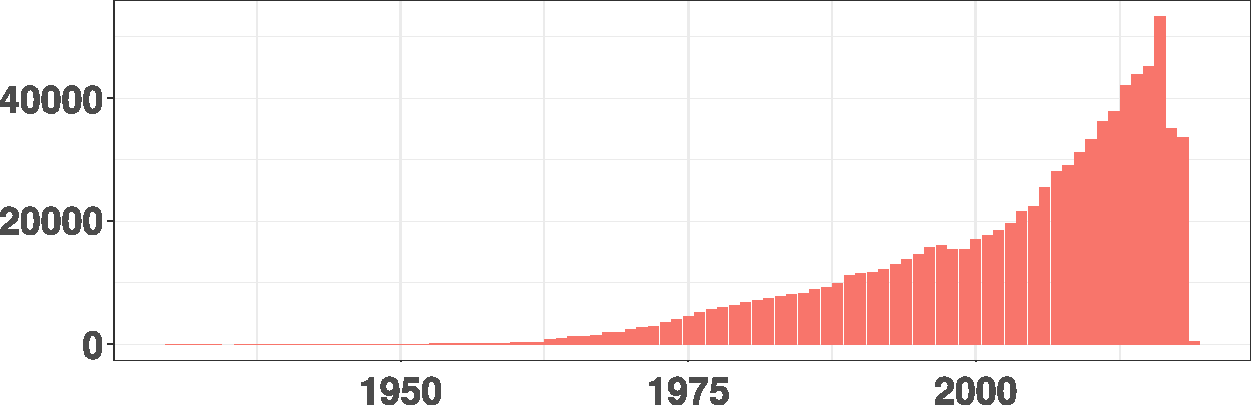
\includegraphics[width=\textwidth]{figures/VYLOMOVA_yearstats_cropped.pdf}
\caption{Statistics on the number of abstracts per year}
\label{fig:year-pubs}
\end{figure}


\subsection{CoCA and CoHA}

The corpus of historical English (CoHA) starts in the 1810s and ends in the early 2000s, comprising 400 million words from 115,000 texts evenly sampled for each decade from fiction, magazines, newspapers, and non-fiction books.

The corpus of contemporary American English (CoCA) covers the period from 1990 till 2019 and contains about 1 billion words from 500,000 texts evenly sampled from spoken, TV shows, academic journals, fiction, magazines, newspapers, and blogs.

For the purpose of the study, we combined the two corpora leaving only the period between 1970 and 2017. We excluded blogs because of the lack of timestamps and additionally removed texts extracted from academic journals to ensure a contrast between academic and non-academic sources for our analyses. 

\subsection{Preprocessing steps}

All corpora were preprocessed in the same way: we removed punctuation, numbers, stop-words and non-English words, did case folding and lemmatization using spaCy.\footnote{\url{https://spacy.io/}. spaCy uses a pre-trained multi-task CNN-based model that takes into account part-of-speech information (i.e. adjective \emph{addicted} will not be transformed into \emph{addict}).}

The resulting corpus of psychology abstracts comprises 73,788,954 tokens from 825,628 texts.
The general domain corpus has 253,597 texts with 237,205,654 tokens in total.

\section{Representation of concepts}\largerpage
We manually associate each concept with a list of most morphologically and semantically related words. For our frequency analysis we sum the corresponding token frequencies.\footnote{As we mentioned above, the corpus contains lemmata only.} We only consider tokens that occurred at least 50 times in each corpus. The final representation of concepts is as follows:

\begin{description}[font=\normalfont]
\item[`Addiction':] \textit{addict}, \textit{addiction}
\item[`Bullying':] \textit{bully}, \textit{bullying}
\item[`Trauma':] \textit{trauma}, \textit{traumatic}, \textit{traumatize}
\item[`Harassment':] \textit{harass}, \textit{harassment}
\item[`Prejudice':] \textit{prejudice}
\end{description}

In order to obtain concept vector representations, we follow the \textsc{distributed dictionary representations} approach proposed in \citet{garten2018dictionaries} which is similar to \citet{mendelsohn2020framework}. More specifically, we represent each concept as a mean vector of the corresponding word vector representations (e.g., `addiction' would be an average of vector representations of \textit{addict} and \textit{addition}).
Unlike \citet{mendelsohn2020framework} we do not assign frequency-based weights to tokens.

\section{Experiments}
\subsection{Frequency-based analysis}
For each of the five concepts we first evaluate their (unigram) frequency distribution over time. We evaluate relative frequencies by normalizing the raw counts by the total number of tokens in each year.\footnote{We also applied a moving average smoothing with window size of 1, i.e. $f_{1972}=(f_{1971}+f_{1972}+f_{1973})/3$.} 

\begin{figure}[p]
  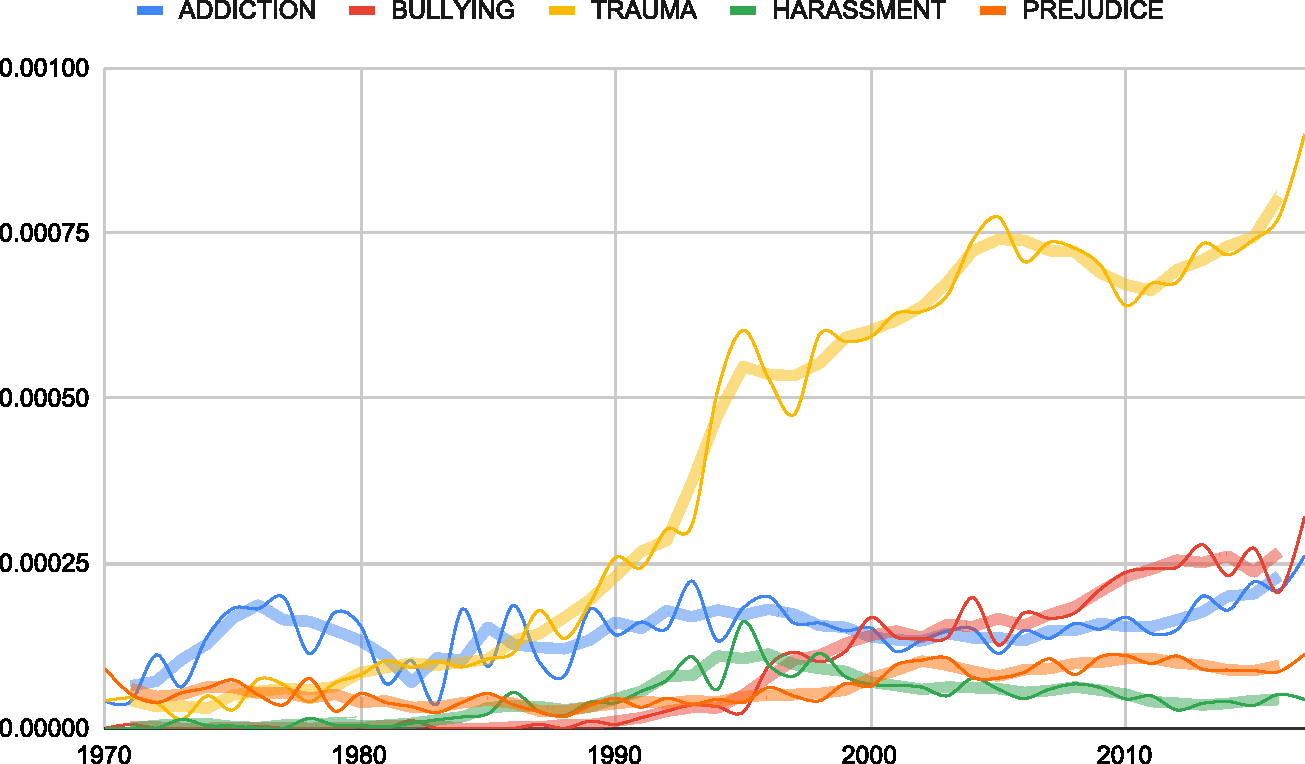
\includegraphics[width=.8\textwidth]{figures/VYLOMOVA_harm-relfreq.pdf}
\caption{Relative concept frequencies based on abstracts from psychology journals. Bold lines correspond to moving average smoothing (window=1).\label{fig:journals-ngrams}}
\end{figure}

\begin{figure}[p]
  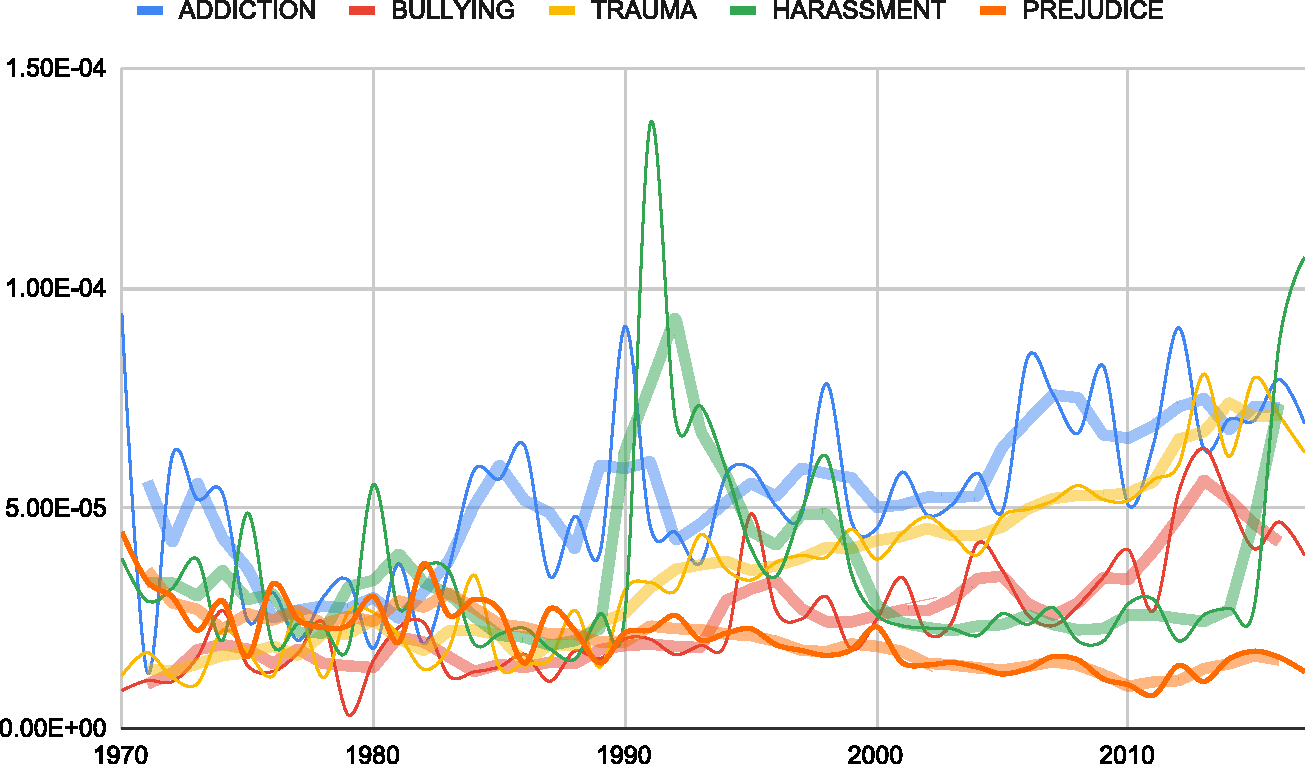
\includegraphics[width=.8\textwidth]{figures/VYLOMOVA_harm-relfreq-coca.pdf}
\caption{Relative concept frequencies based on general domain corpus. Bold lines correspond to moving average smoothing (window=1).\label{fig:coca-ngrams}}
\end{figure}

As Figure~\ref{fig:journals-ngrams} demonstrates, in the psychology domain all concepts demonstrate relative increase in frequency: `trauma' exhibits the steepest slope, `bullying' gradually raises since the 1990s, and `harassment' has its peak in the mid-1990s. `Addiction' and `prejudice' present the lowest changes in relative fre\-quen\-cy. The results obtained on CoCA/COhA (Figure~\ref{fig:coca-ngrams}) are more unsteady and labile: `trauma' rises over time but much less rapidly compared to the psychology literature, relative frequencies of `addiction' and `bullying' increase over time. `Harassment' also demonstrates the highest usage in the early 1990s while `prejudice' slightly declines.
Does the increase in the frequency of `trauma' imply that it has broadened over time, i.e. its usages expanded to new contexts, especially in psychology literature?  On the other hand, `trauma' exhibits the highest usage among the five concepts in psychology literature, so ``the law of conformity'' \citep{hamilton-etal-2016-diachronic} would
predict that it should change slower. `Harassment' presents the lowest raw frequencies throughout most time periods but has risen in the mid-nineties. Would this imply that `harassment' changed its meanings faster and achieved the highest breadth in the nineties? 

\begin{figure}[p]
  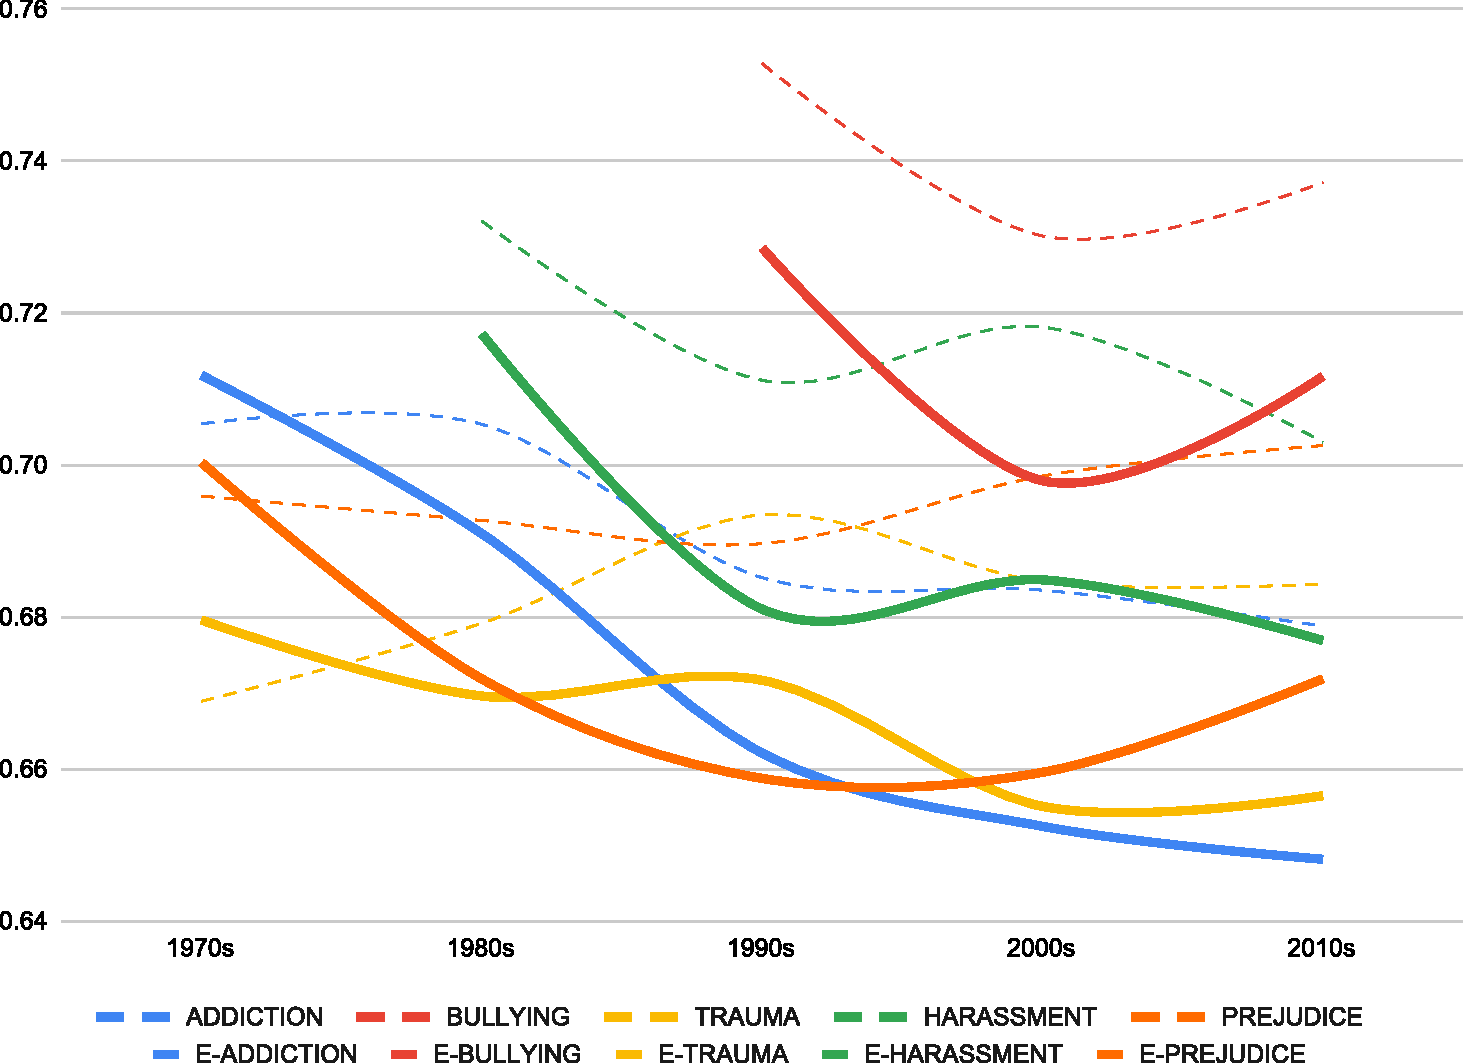
\includegraphics[width=.8\textwidth]{figures/VYLOMOVA_context-sim-psychol.pdf}
\caption{Mean cosine similarities (polynomial smoothing) over five decades (psychology abstracts corpus). Bold and dashed lines correspond to epoch-specific (e-*) and global (static) embeddings, respectively. \label{fig:avg-cos-sim-psych}}
\end{figure}

\begin{figure}[p]
  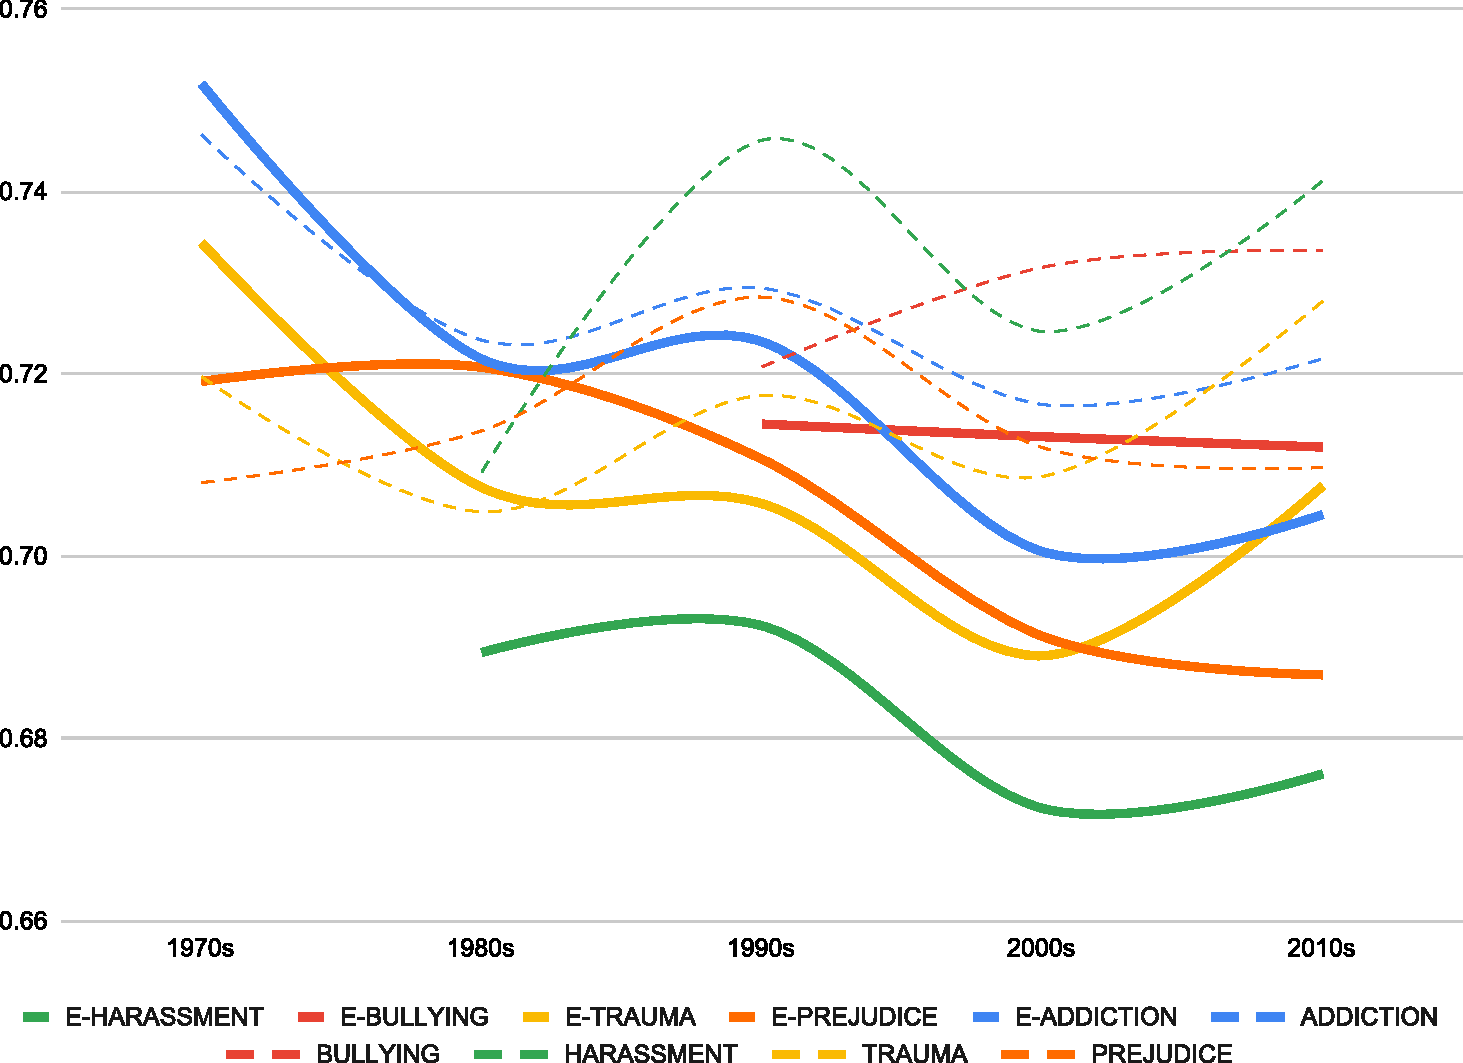
\includegraphics[width=.8\textwidth]{figures/VYLOMOVA_context-sim-coca.pdf}
\caption{Mean cosine similarities (polynomial smoothing) over five decades (general domain corpus). Bold and dashed lines correspond to epoch-specific (e-*) and global (static) embeddings, respectively.\label{fig:avg-cos-sim-cocha}}
\end{figure}


In the next section, we adapt two diachronic variations of word2vec \citep{mikolov2013-distributed} to quantify semantic change over time.
We first train a type-based model conceptually similar to the one proposed in \citet{mendelsohn2020framework}. We use the type-level embeddings to obtain token-level (sentence-specific) representations which are further utilized to measure semantic breadth in each epoch. We then take a closer look at the type-level epoch-specific embeddings to study \emph{how exactly} concepts changed. Such models have previously shown their utility at capturing semantic changes over time \citep{tahmasebi2018survey,kutuzov-etal-2018-diachronic} and do not require vector space alignment \citep[which, as has been previously shown, leads to noise;][]{dubossarsky-etal-2019-time}.  


\subsection{Diachronic word2vec}
We first train a \emph{type-level} word2vec skip-gram model.\footnote{Using \url{https://radimrehurek.com/gensim/}.} In terms of hyper-param\-e\-ter setting we follow that of \citet{mendelsohn2020framework}. Since we mainly focus on semantic changes, we set the context window size to 10 to better capture semantics and associations \citep{agirre2009study}. We also do not consider tokens that occur less than 5 times over the whole corpus. We train the model on the whole corpus for 10 iterations (obtaining \emph{global}--static embeddings). We then use the global embeddings to initialize epoch-specific models that we continue training on each epoch's data independently for another 10 iterations. We split time periods by decades.\footnote{Due to an insufficient amount of data for earlier time periods, we train the models only on the following time frames: 1980--1989, 1990--1999, 2000--2009, 2010--2017.}   


\subsubsection{Token-level embeddings}
In order to obtain token-level embeddings, the resulting (global and epoch-spe\-cif\-ic) embeddings are then contextualized for each decade starting the 1970s and finishing the 2010s. This part of experiments is based on the method proposed by \citet{sagi-etal-2009-semantic} except that we use the word2vec model \citep{mikolov2013-distributed} rather than LSA \citep{landauer2013handbook} (therefore, we refer to it as ``neural parameterization of Sagi et al.'s model''). 

More specifically, in order to get sentence-specific vector representations for each concept in  a certain decade, we randomly sample a number of its sentential occurrences\footnote{We set the number to 50. We use all sentential instances if the concept occurs less than 50 times during the epoch (having 20 as a minimum)} from the respective period, then extract contextual tokens found within the pre-set window size.\footnote{We set the window size to be 3, 7, 9 tokens at each side and found that 9 provides smoother results, so we used this setting throughout.}
The final sentence-specific representation is a bag-of-words, i.e. it is an average over corresponding token representations.
Following \citet{sagi-etal-2009-semantic}, in order to estimate the semantic breadth of a word, we evaluate pair-wise cosine similarities across all the sentence-specific representations.   
To reduce any biases, we repeat the above sentence sampling process 10 times. The final mean values for cosine similarities for both types of models, global and epoch-specific, in the psychology and general domains are presented in Figures~\ref{fig:avg-cos-sim-psych} and~\ref{fig:avg-cos-sim-cocha}. The figures also illustrate that epoch-specific embeddings (marked as bold) provide more robust results, and we will mainly rely on them in our study.

\begin{sloppypar}
 The five concepts behave differently over time. For instance, `trauma', although becoming frequently used in the psychology corpus, has only broadened its meaning slightly and has stayed quite a ``broad'' concept. In CoCA/CoHA \emph{trauma} does not appear much before the 1990s.\footnote{I.e. it is much less represented in CoHA.} Figure~\ref{fig:avg-cos-sim-cocha} presents two slopes; the first one can be possibly explained by the difference in its frequency distribution in CoCA and COhA, while the second one is due to its breadth changes.
The notion of `harassment', on the other hand, has the steepest slope between the 1980s and the 1990s, and then it stabilizes in its contextual usages. The highest contextual similarity in the 1980s can be partially attributed to relatively few usage instances in psychology corpus during this period. In CoCA/CoHA, frequency of `harassment' has a drastic leap in the 1990s but, as Figure~\ref{fig:avg-cos-sim-cocha} shows; it does not affect its breadth when compared to the 1980s, although it becomes broader in the the 2000s (its usage frequency also decreases). The concept of `bullying' has been constantly increasing in its relative usage frequency in the psychology literature, although its semantics presents a more complex pattern: it broadened from the 1990s to the 2000s, and then narrowed in the 2010s. In CoCA/CoHA the usage of `bullying' was more stable and did not significantly change in frequency and semantics. Similarly, `addiction' stayed within the same frequency range after the 1990s (although being much less frequent in the 1970s and the 1980s), and its breadth slightly increased since then. In the psychology domain its semantic breadth changes are more drastic: `addiction' has been gradually becoming broader since the 1970s due to its expansion to new behavior types.  
Finally, `prejudice', the concept that was not widely used before the 2000s in both corpora,\footnote{It appears less than 100 times a year before early 2000s.} behaves differently in the general and psychology domains: in psychology abstracts it narrows down in the 2010s while in CoCA/CoHA it continues to expand its meaning.
The results support the findings obtained for the LSA-based model in \citet{vylomova-etal-2019-evaluation}. The next part of the chapter investigates how exactly the meanings changed.
\end{sloppypar}

\subsubsection{Type-level embeddings}
We now use the obtained epoch-specific \emph{type-level} embeddings to run a detailed study of concept change.

Following \citet{hamilton-etal-2016-diachronic}, we consider two metrics to evaluate semantic changes over time:

\begin{enumerate}
\item \textit{Semantic displacement}, which shows to what extent a concept has semantically changed during a certain time period. This is quantified as cosine distance between the word embeddings from the corresponding time periods, i.e. $\text{cos-dist}(\mathbf{w}^t, \mathbf{w}^{t+\delta})$.

Figure~\ref{fig:cos-dist-years} shows the results of the semantic displacement evaluation and confirms our observations made earlier using the model from \citet{sagi-etal-2009-semantic}.
Concepts such as `trauma', `bullying', `prejudice' change similarly in the psychology and general domain corpora. The largest gaps are observed in the case of `addiction'.


\item \textit{Pair-wise similarity time-series}, which is quantified as
\[ s^{(t)}(w_i,w_j)=\text{cos-sim}(\mathbf{w}^t_i,\mathbf{w}^t_j) \]

and measures how cosine similarity between words $w_i$ and $w_j$ changes over time period $(t; t+\delta)$.
For each concept we first constructed a list of words which the concept most often co-occurred with within each time period. Then we calculated cosine similarity between the concept and every word from the list for each decade. We will now discuss changes in each concept individually. 

\end{enumerate}

\begin{figure}
  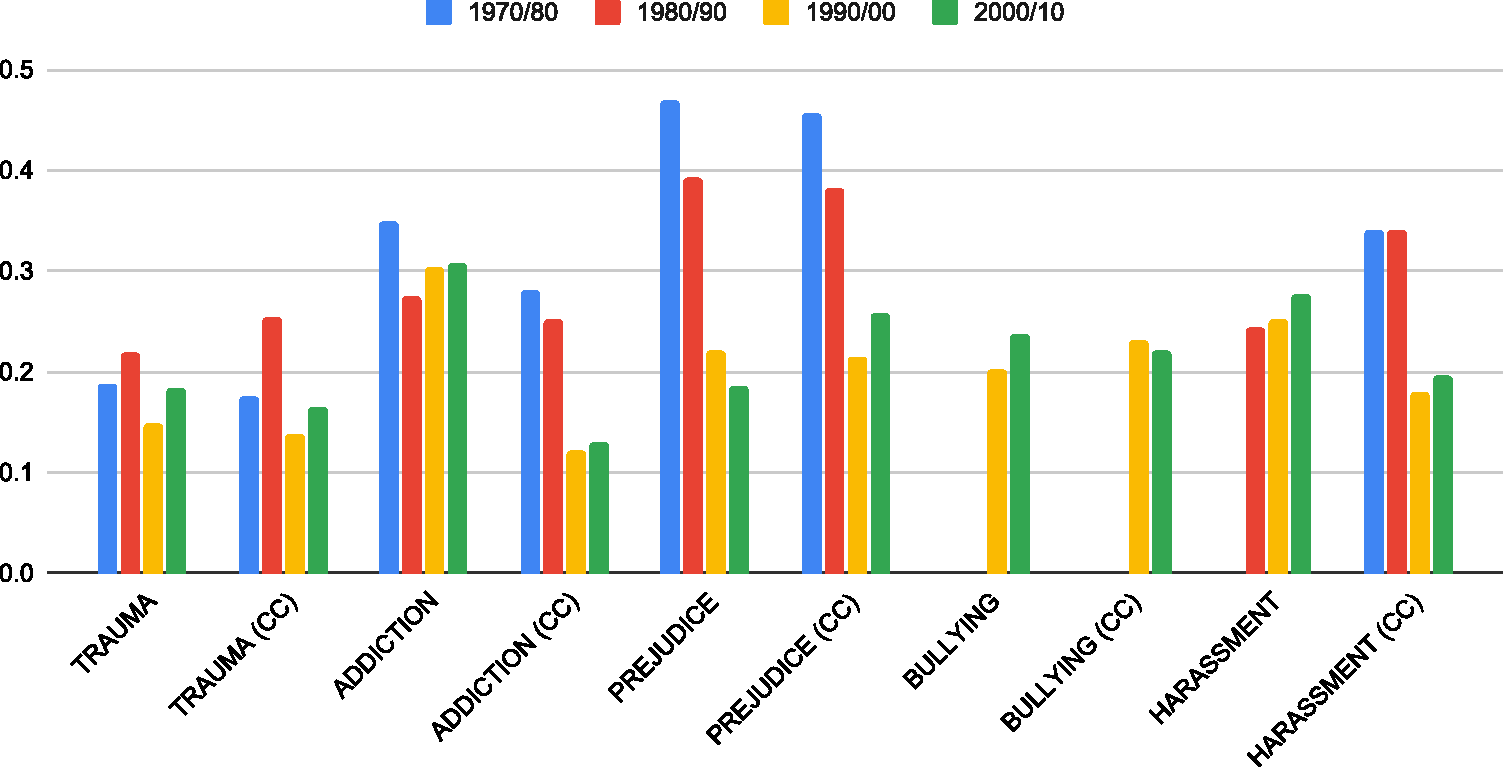
\includegraphics[width=\textwidth,keepaspectratio]{figures/VYLOMOVA_distances-between-epochs-1.pdf}
\caption{Cosine distances between decades in the psychology and \mbox{CoCA/CoHA} (CC) domains}
\label{fig:cos-dist-years}
\end{figure}

\subsubsubsection{`Trauma'}
\begin{sloppypar}
As Figure~\ref{fig:w2v-cos-sim-trauma} illustrates, `trauma' has undergone more significant meaning changes in the psychology literature than in CoCA/CoHA where it preserves most associations since the 1990s. More specifically, in the psychology corpus, we observe a clear shift from \emph{physical} to \emph{psychological}. Although its relatedness to \emph{severe} is still more prevalent than \emph{mild}, they both increase their similarity to `trauma' over time. In both corpora, `trauma' started moving away from \emph{childhood} in the 2000s.
\end{sloppypar}

\begin{figure}[H]
   \begin{subfigure}[b]{.5\linewidth}
        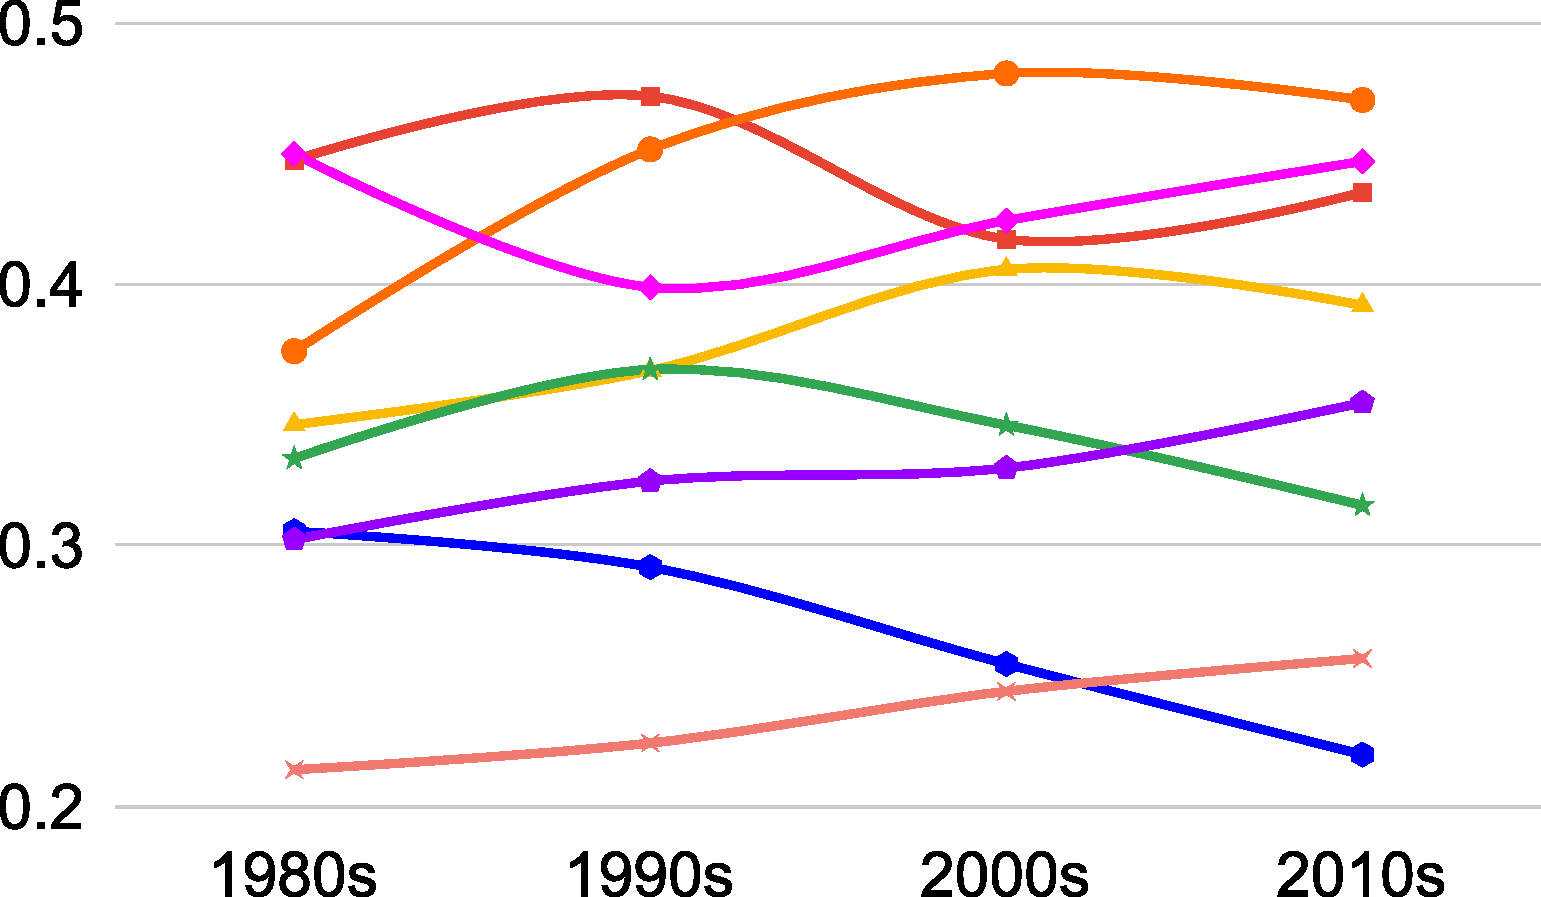
\includegraphics[width=\textwidth]{figures/VYLOMOVA_trauma-psych.pdf}
        \caption{Psychology}
    \end{subfigure}\begin{subfigure}[b]{.5\linewidth}
        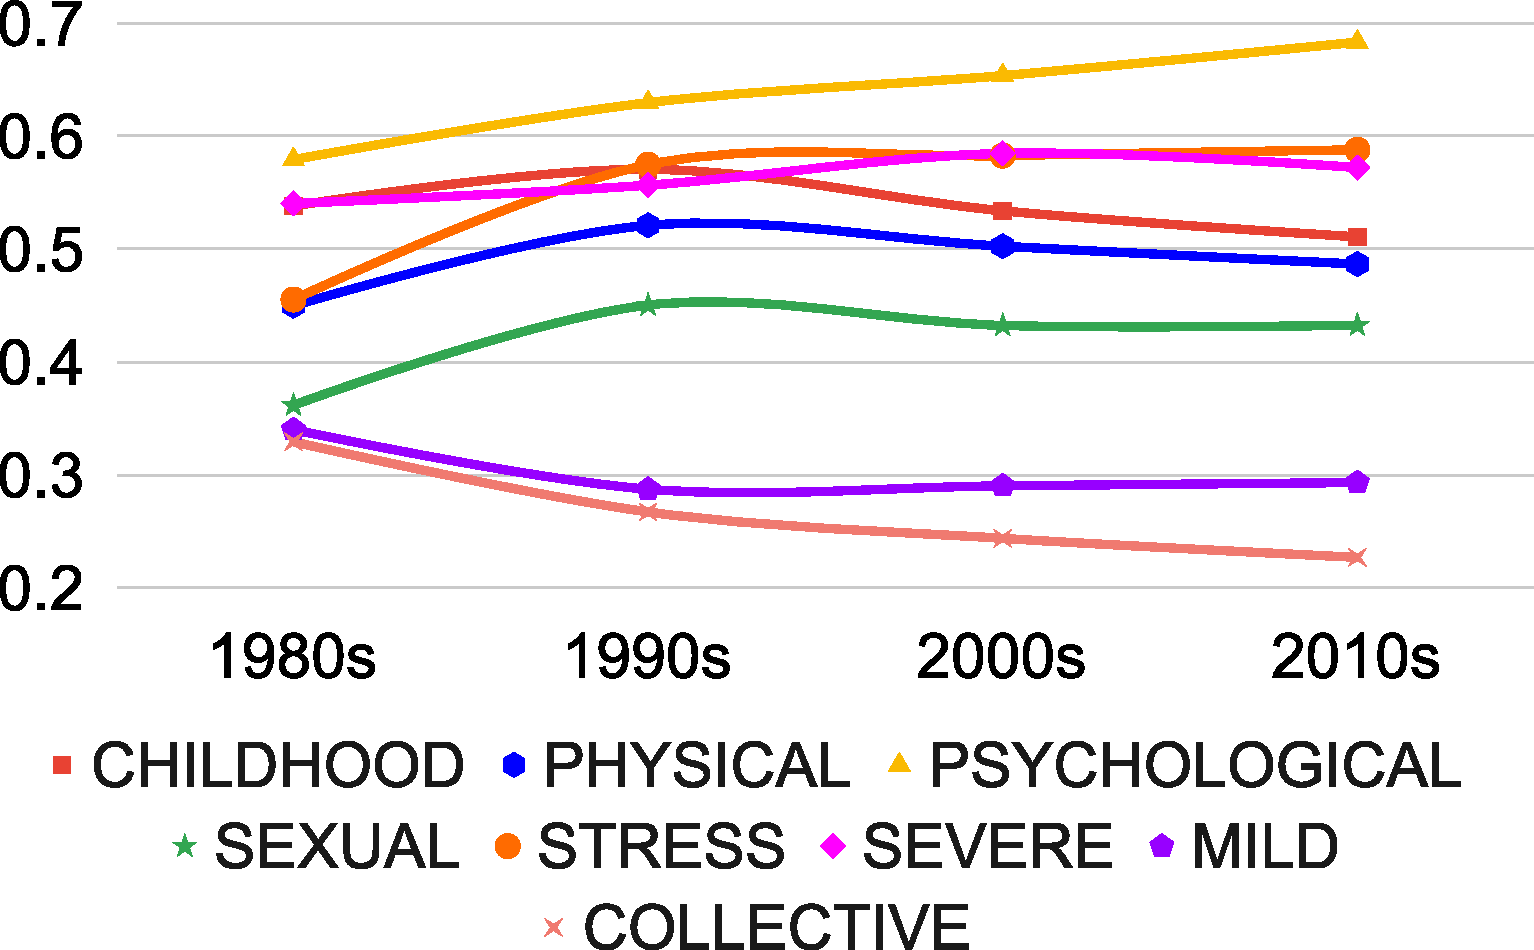
\includegraphics[width=\textwidth]{figures/VYLOMOVA_trauma-coca-1.pdf}
        \caption{General Domain (CoCA+CoHA)}
    \end{subfigure}%
\caption{`Trauma'. Cosine similarities over four decades}
\label{fig:w2v-cos-sim-trauma}
\end{figure}

Table~\ref{tab:trauma-nns} lists its top nearest neighbors in both corpora: `trauma' stays strongly associated with `PTSD'. In the general domain it is associated with \textit{horrific} and \textit{suffer}, and its relatedness to the latter increases over time. During the 1990s--2000s `trauma' becomes more \textit{emotional} and \textit{psychological}, which is in line with \citet{haslam2020concept}'s findings that show
changes in the relative frequency of trauma-related concepts in the massive Google Books corpus from 1960 to 2008. They found that during the 1990s the term \textit{psychological trauma} rose most steeply. 

\begin{table}
\footnotesize
\caption{`Trauma'. Top-10 nearest neighbors\label{tab:trauma-nns}}
\begin{tabular}{llll}
\lsptoprule
\multicolumn{4}{c}{Psychology}\\
\multicolumn{1}{c}{1980s} & \multicolumn{1}{c}{1990s}  & \multicolumn{1}{c}{2000s} & \multicolumn{1}{c}{2010s}\\\midrule
humbling&posttraumatic&ptsd&posttraumatic              \\   
posttraumatic&ptsd&posttraumatic&ptsd                  \\   
retraumatization&survivor&traumatization&traumatization\\   
traumatized&posttrauma&traumatized&aftermath           \\   
traumatizing&retraumatization&traumatizing&dissociative\\   
traumatogenic&injury&desnos&peritraumatic              \\   
terrifying&traumatized&torture&traumatized             \\   
debility&atrocity&survivor&traumatically               \\   
traumatise&traumatization&dissociative&posttrauma      \\   
survivor&dissociative&posttrauma&atraumatic            \\   
traumatization&sequelae&flashback&traumatizing         \\   
unassimilable&ptsdlike&nontraumatize&pts               \\   
torture&ptds&retraumatization&refugee                  \\   
traumatised&peritrauma&peritraumatic&mtbi              \\   
hypnoanalysis&desnos&nontrauma&telecommunicator        \\   
traumatolytic&psychotraumatic&lifethreat&ptss          \\   
keilson&torture&holocaust&sequelae                     \\   
flashback&reexperience&nontraumatic&flashback          \\   
psychotraumatic&lasc&traumatise&postraumatic           \\   
hypnoid&traumatologist&ptes&desnos                     \\ \midrule
\multicolumn{4}{c}{CoCA/CoHA}\\
\multicolumn{1}{c}{1980s} & \multicolumn{1}{c}{1990s}  & \multicolumn{1}{c}{2000s} & \multicolumn{1}{c}{2010s}\\\midrule
salomo&ptsd&ptsd&ptsd\\
posttraumatic&spiegle&posttraumatic&psychological\\
hyperarousal&psychological&traumatization&boehnlein\\
traumatization&emotional&psychological&posttraumatic\\
reliving&posttraumatic&emotional&hyperarousal\\
traumatized&horrific&horrific&suffer\\
indentify&psychosis&suffer&traumatization\\
louxes&traumatization&traumatizing&horrific\\
clinginess&suffer&experiencing&emotional\\
emotional&victim&hyperarousal&experiencing\\
przekop&disorder&spiegle&spiegle\\
brayme&sexualizing&przekop&injury\\
experiencing&hyperarousal&disorder&victim\\
ptsd&brayme&victim&traumatizing\\
boehnlein&abuse&painful&disorder\\
rohrbacher&syndrome&brayme&traumatically\\
spiegle&therapist&hospitalize&csf2\\
traumatizing&cope&severe&scurfield\\
csf2&boehnlein&psychiatric&przekop\\
traumatically&gavigan&tbi&yancosek\\  
\lspbottomrule
\end{tabular}
\end{table}

\begin{table}
\footnotesize
\caption{`Addiction'. Top-10 nearest neighbors\label{tab:addiction-nns}}
\begin{tabular}{llll}
\lsptoprule
\multicolumn{4}{c}{Psychology}\\
\multicolumn{1}{c}{1980s} & \multicolumn{1}{c}{1990s}  & \multicolumn{1}{c}{2000s} & \multicolumn{1}{c}{2010s}\\\midrule
heroin&addicted&addicted&addictive         \\   
addicted&addictive&opiate&addicted         \\   
narcotic&abuser&abuser&dependence          \\   
methadone&heroin&heroin&heroin             \\   
nonopiate&substance&addictive&mmt          \\   
illicit&dependence&drug&craving            \\   
nonaddiction&alcoholic&dependence&internet \\   
drug&drug&substance&opiate                 \\   
opiate&opiate&methadone&opioid             \\   
alcoholism&methadone&abstinence&drug       \\   
polysubstance&cocaine&cocaine&abuser       \\   
detoxification&alcoholism&detoxify&cybersex\\   
nonaddicte&gambler&illicit&substance       \\   
alcohol&crack&detoxification&crave         \\   
abuser&abuse&abuse&problematic             \\   
detox&nonaddicte&crave&yfas                \\   
mmt&coaddict&craving&detoxification        \\   
cocaine&alcohol&abstinent&igd              \\   
polydrug&detoxification&opioid&abstinent   \\   
nonnarcotic&mmt&alcoholism&gaming          \\\midrule
\multicolumn{4}{c}{CoCA/CoHA}\\
\multicolumn{1}{c}{1980s} & \multicolumn{1}{c}{1990s}  & \multicolumn{1}{c}{2000s} & \multicolumn{1}{c}{2010s}\\\midrule
drug&addicted&addicted&addicted\\
heroin&heroin&heroin&heroin\\
pcp&drug&addictive&opiate\\
abuser&abuser&alcoholism&opioid\\
methadone&alcoholic&meth&methadone\\
cocaine&cocaine&cocaine&alcoholism\\
marijuana&alcoholism&alcoholic&rehab\\
amphetamine&methadone&abuser&addictive\\
addictive&alcohol&rehab&alcoholic\\
alcohol&addictive&drug&suboxone\\
opioid&rehab&oxycontin&drug\\
alcoholic&oxycontin&methamphetamine&painkiller\\
quashen&marijuana&waismann&quashen\\
cannabis&abuse&medicate&overdose\\
opiod&henningfield&methadone&alcohol\\
alcoholism&buprenorphine&alcohol&vivitrol\\
methamphetamine&12step&quashen&acamprosate\\
mdma&quashen&buprenorphine&relapse\\
mcshin&relapse&12step&sober\\
addicted&addicting&relapse&oxycontin\\   
\lspbottomrule
\end{tabular}
\end{table}


\subsubsubsection{`Addiction'}
`Addiction' demonstrates a remarkable shift in the psychology literature from a substance-related concept in the 1980s to a behavior-related concept in the 2010s, but this pattern is less evident in CoCA/CoHA (see Figure~\ref{fig:w2v-cos-sim-addiction} and Table~\ref{tab:addiction-nns}).
More specifically, we observe that the concept moved away from  `narcotic'-related meanings towards \textit{gaming}, \textit{Internet}, \textit{cybersex}, and \textit{smartphone}.  
The findings confirm earlier observations done by \citet{vylomova-etal-2019-evaluation} who used the diachronic language model from \citet{hamilton-etal-2016-diachronic}.
In psychology literature, such conceptual expansion of `addiction' had prompted and induced adaptation of a range of psychosocial treatments to be used to treat gambling, internet, and sexual addictions \citep{yau2015gambling}.

\begin{figure}[H]
  \begin{subfigure}[b]{.5\linewidth}
        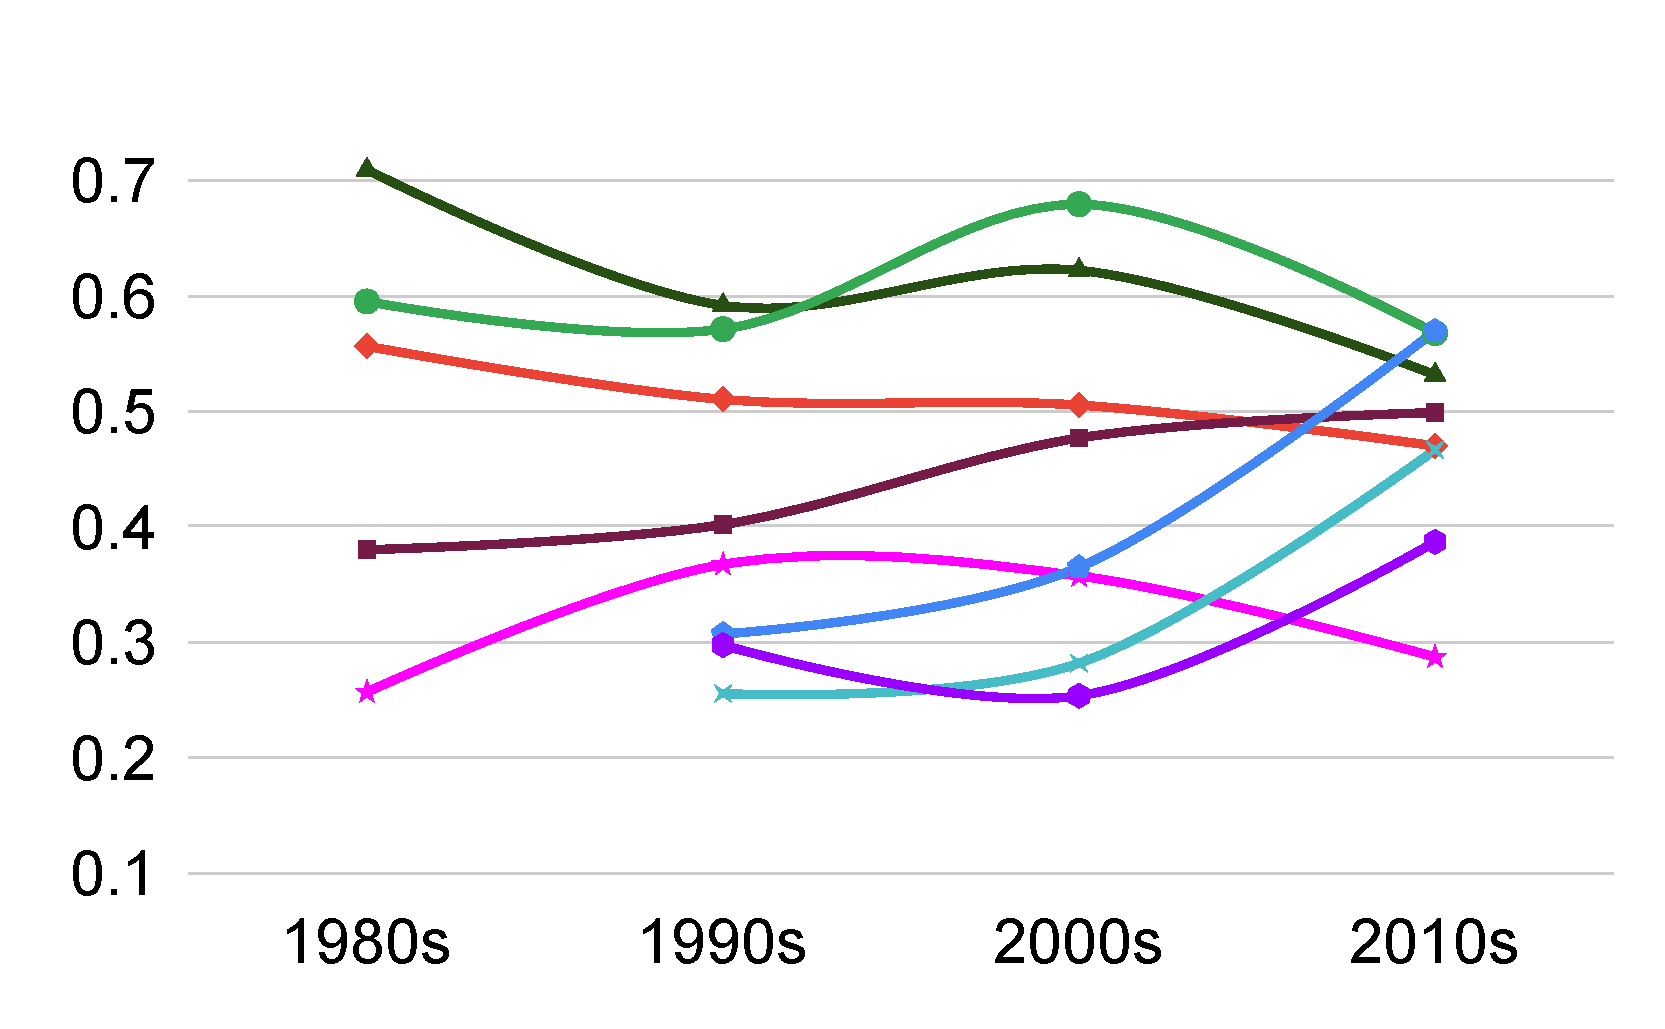
\includegraphics[width=\textwidth]{figures/VYLOMOVA_addiction-psych.pdf}
        \caption{Psychology}
        \end{subfigure}\begin{subfigure}[b]{.5\linewidth}
        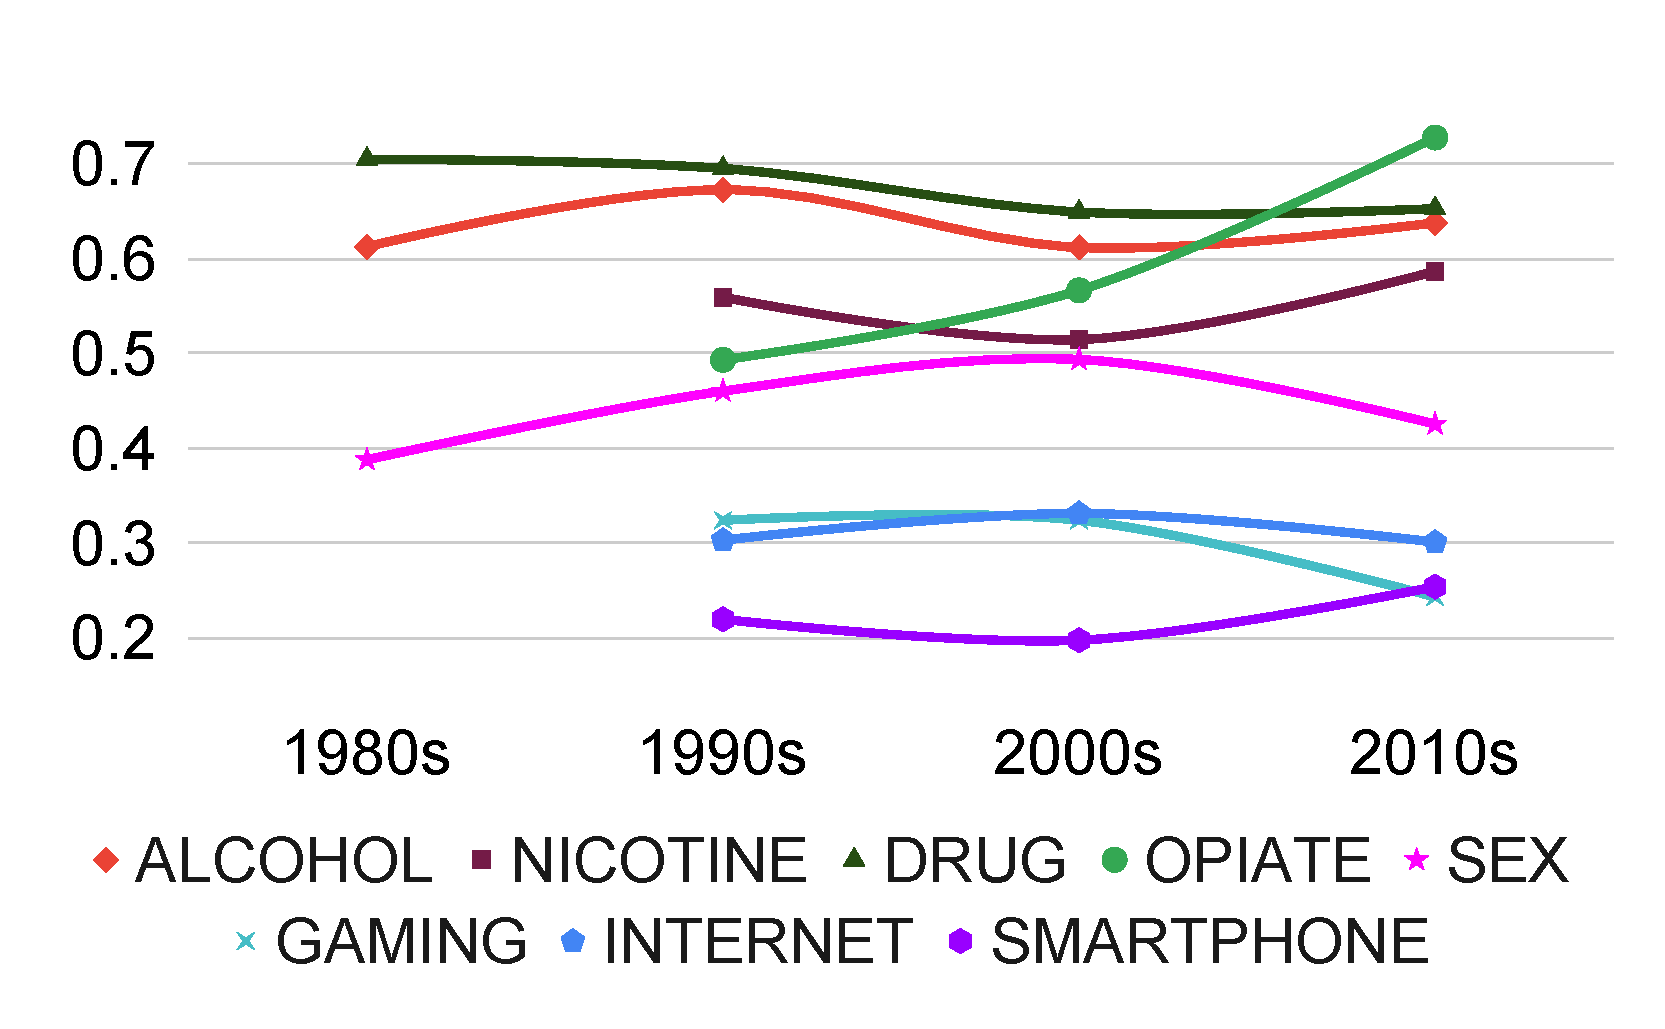
\includegraphics[width=\textwidth]{figures/VYLOMOVA_addiction-coca.pdf}
        \caption{General Domain (CoCA+CoHA)}
        \end{subfigure}
\caption{`Addiction'. Cosine similarities over four decades.\label{fig:w2v-cos-sim-addiction}}
\end{figure}

In the general domain corpora, initial associations of `addiction' are more stable over time, and the similarity to \textit{opiate} even increases during the last two decades.
In both domains, `addiction' becomes less associated with \textit{abuse} and \textit{abuser}: the similarity drops by 0.1--0.15 since the 1990s and 2000s.

\subsubsubsection{`Harassment'}
In both corpora, usage of `harassment' increases in the 1990s, and the 1980s do not contain enough instances to obtain reliable embeddings.
As Figure~\ref{fig:w2v-cos-sim-harassment} shows, `harassment' is highly related to \textit{sexual} in both domains.
In the psychology literature `harassment' moves away from \textit{workplace} towards \textit{online} and \textit{cyber} (increasing its relatedness to `bullying'). In the general domain there are fewer marked changes across decades. The relationship to \textit{online} and \textit{cyber} is weaker than in the psychology corpus and, in contrast to that corpus, `harassment' is more associated with \textit{verbal} than \textit{physical}.\footnote{This is probably due to `physical' being the default characteristic of `harassment' and usually is not explicitly marked.} These findings point to similarities across the corpora, but we observe a more rapidly growing preoccupation of psychology with digitally mediated forms of harassment.

\begin{figure}[H]
  \begin{subfigure}[b]{.5\linewidth}
        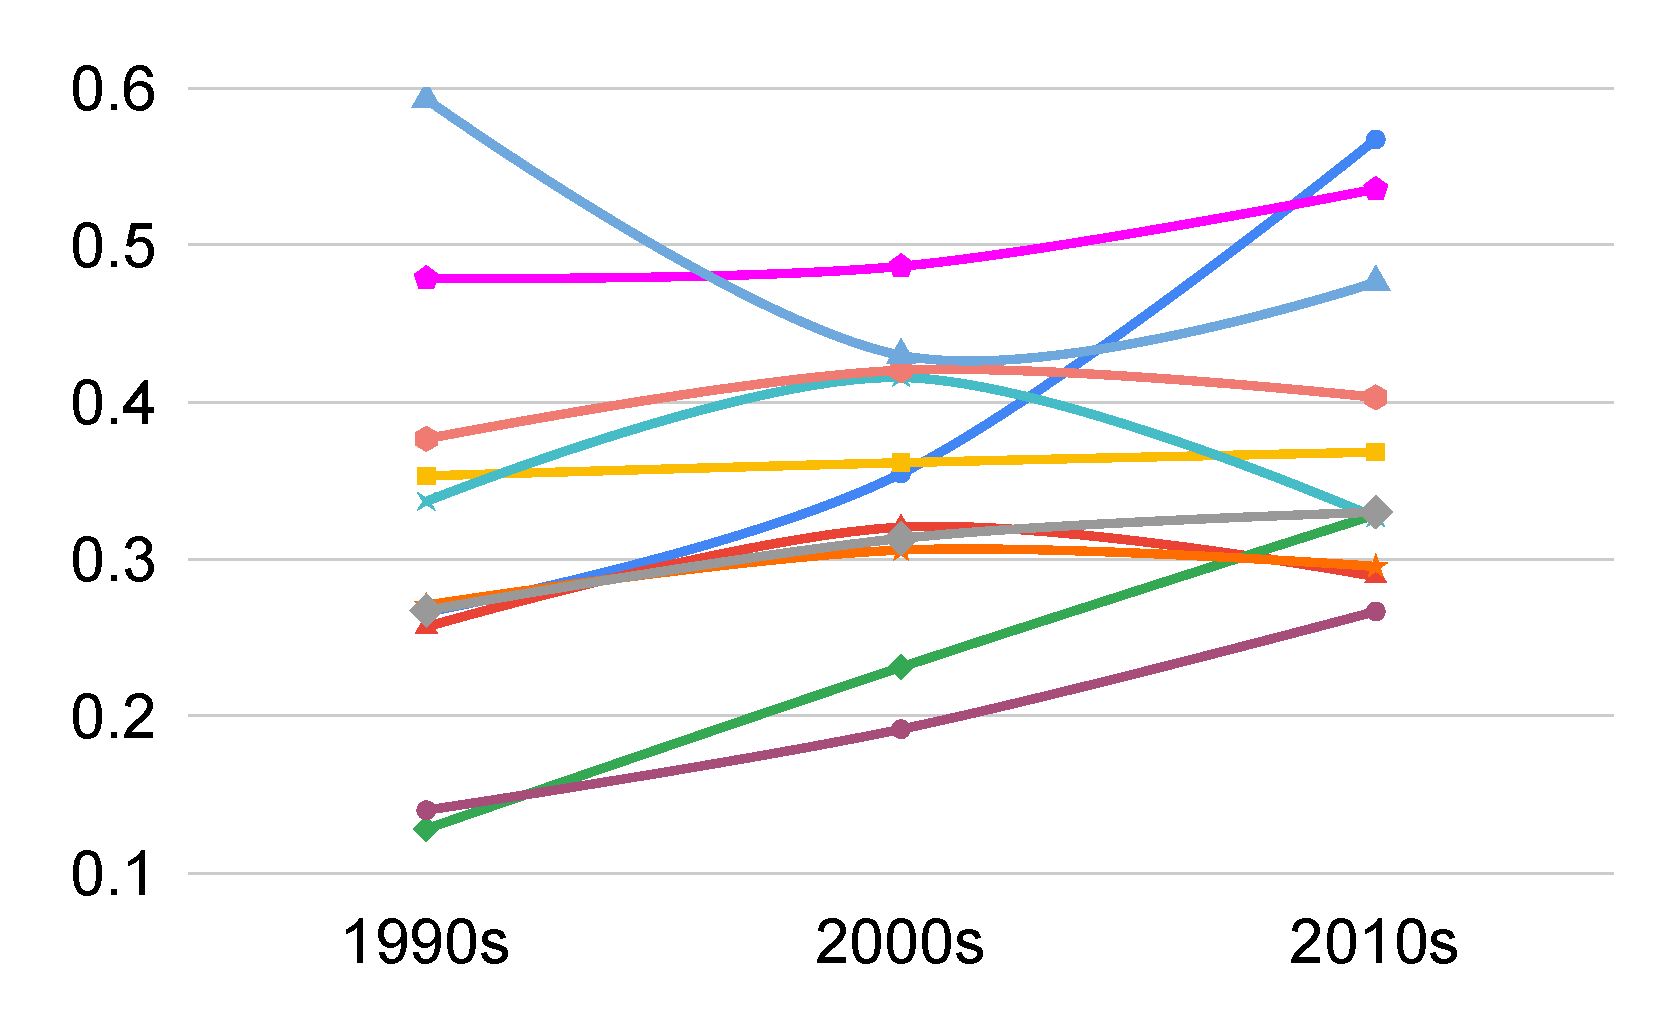
\includegraphics[width=\textwidth]{figures/VYLOMOVA_harassment-psych.pdf}
        \caption{Psychology}
        \end{subfigure}\begin{subfigure}[b]{.5\linewidth}
        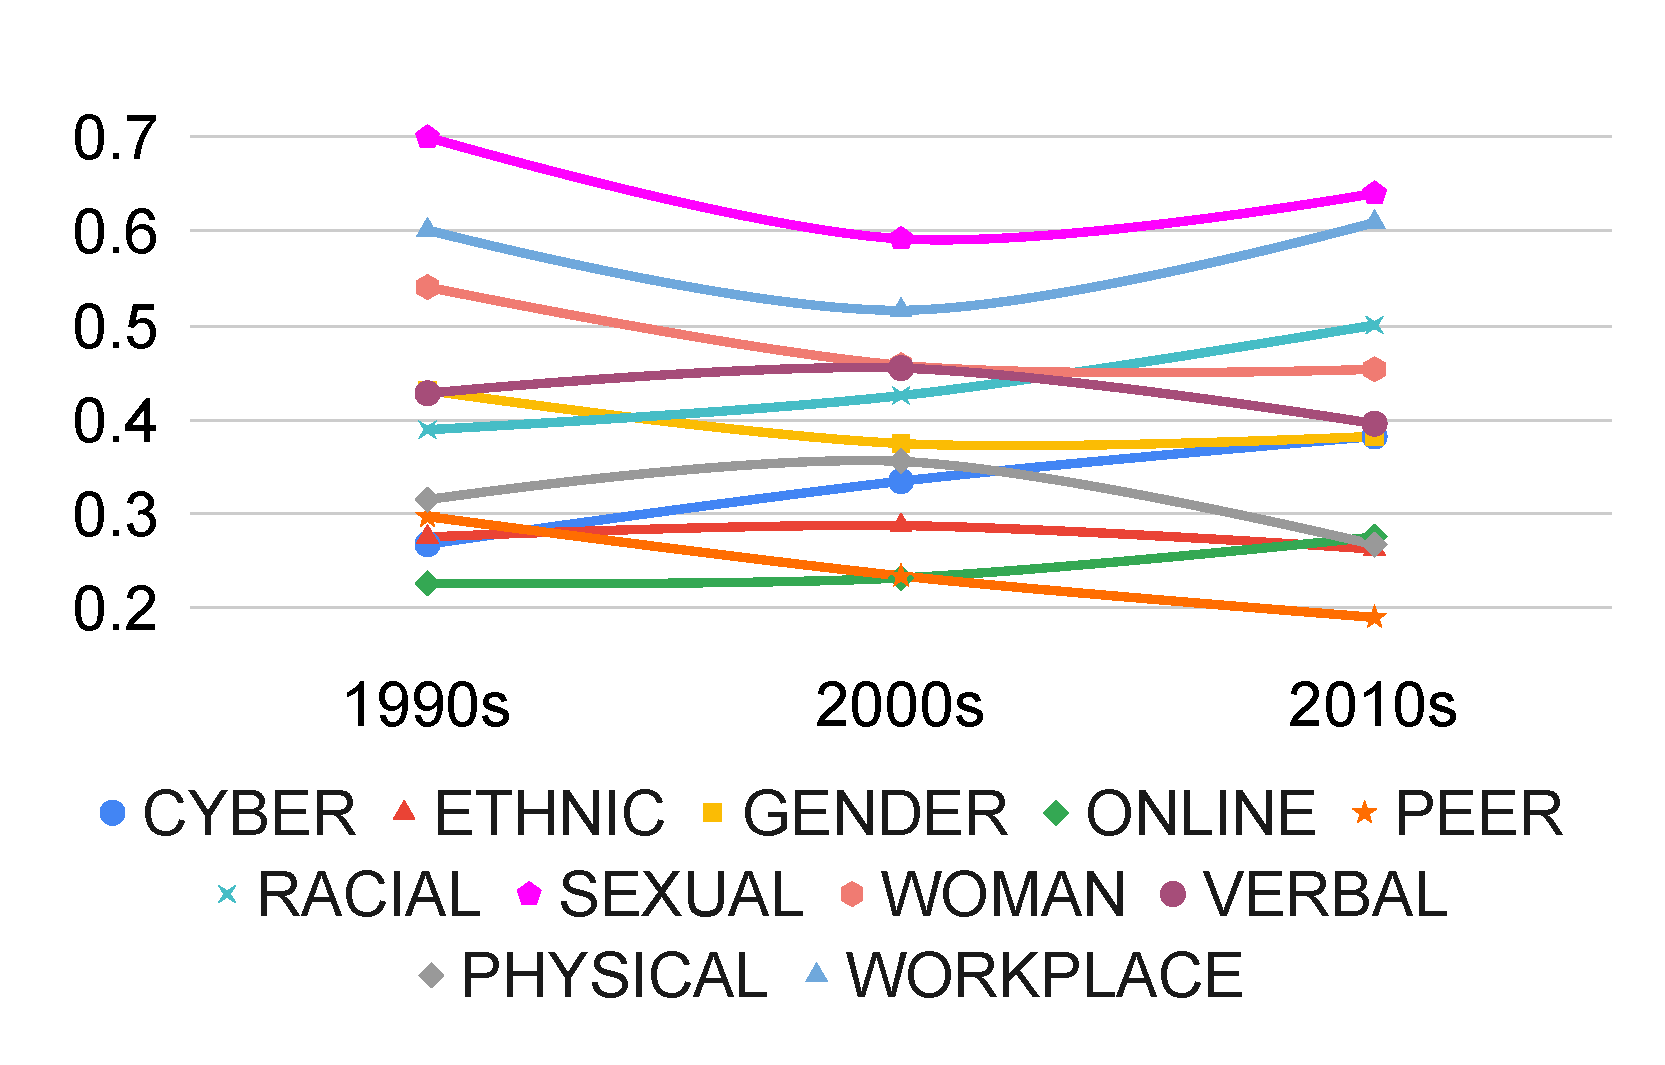
\includegraphics[width=\textwidth]{figures/VYLOMOVA_harassment-cos-sim-cocha.pdf}
        \caption{General Domain (CoCA+CoHA)}
        \end{subfigure}
 \caption{`Harassment'. Cosine similarities over three decades\label{fig:w2v-cos-sim-harassment}}
\end{figure}

By looking at the nearest neighbors space shown in Table~\ref{tab:harassment-nns}, we additionally notice substantial differences in the two domains: `harassment' in psychology preserves its emphasis on \textit{victimization}, the act or process of singling someone out for cruel or unfair treatment, typically through physical or emotional abuse,\footnote{The definition provided in \url{https://dictionary.apa.org/victimization}.} while increases that of \emph{perpetration}.
During the 2000s--2010s it reduced its relatedness to \textit{violence}. The general domain treats the concept of `harassment' in a somewhat more legalistic frame, as a form of \textit{misconduct} that is tightly associated with \textit{allegation}, \textit{complaint}, \textit{accusation}, and \textit{abuse}. 

\begin{table}
\footnotesize
\caption{`Harassment'. Top-10 nearest neighbors\label{tab:harassment-nns}}
 \begin{tabular}{lll}
  \lsptoprule
  \multicolumn{3}{c}{Psychology}\\
 \multicolumn{1}{c}{1990s}  & \multicolumn{1}{c}{2000s} & \multicolumn{1}{c}{2010s}\\
  \midrule
harasser&harasser&harasser           \\ 
workplace&victimization&victimization\\ 
contrapower&contrapower&cyber        \\ 
neosh&uncivil&assault                \\ 
harassing&assault&bullying           \\ 
uncivil&victim&perpetration          \\ 
coercion&bullying&victimize          \\ 
unprofessional&perpetrator&bully     \\ 
assault&lsh&victim                   \\ 
nonharasse&victimize&perpetrate      \\ 
gutek&violence&bystander             \\ 
rape&perpetration&homophobic         \\ 
sexualized&perpetrate&cyberbullying  \\ 
nonheterosexist&rape&incivility      \\ 
sexual&bully&insinuation             \\ 
coercive&lgbts&heterosexist          \\ 
employee&harassing&contrapower       \\ 
perpetrator&cyberstalking&cyberbullye\\ 
incident&socialsexual&sexual         \\ 
intragender&cyberbullye&violence     \\\midrule
\multicolumn{3}{c}{CoCA/CoHA}\\
\multicolumn{1}{c}{1990s}  & \multicolumn{1}{c}{2000s} & \multicolumn{1}{c}{2010s}\\\midrule
harasser&complaint&harasser\\
sexual&accuse&allegation\\
misconduct&complain&assault\\
complaint&intimidate&sexual\\
allege&assault&accusation\\
eeoc&intimidation&allege\\
accuser&allegation&complaint\\
sexually&harasser&workplace\\
allegation&misconduct&accuser\\
accuse&abuse&accuse\\
accusation&abusive&misconduct\\
lawsuit&threaten&rape\\
assault&accusation&intimidation\\
discrimination&renaye&lawsuit\\
incident&sue&harassing\\
abusive&discrimination&alleged\\
workplace&allege&defamation\\
abuse&sexual&abuse\\
rape&sexually&bullying\\
intimidation&mutziger&mistreatment\\
\lspbottomrule
\end{tabular}
\end{table}

\begin{table}
\footnotesize
\caption{`Bullying'. Top-10 nearest neighbors\label{tab:bullying-nns}}
 \begin{tabular}{lll}
  \lsptoprule
  \multicolumn{3}{c}{Psychology}\\
 \multicolumn{1}{c}{1990s}  & \multicolumn{1}{c}{2000s} & \multicolumn{1}{c}{2010s}\\\midrule
victimisation&bullyvictim&cyberbullying         \\  
victimise&victimization&cyberbullye             \\  
cyberbullying&cyberbullying&victimization       \\  
olweus&victimisation&cyber                      \\  
bullyvictim&cyberbullye&victimisation           \\  
antibullying&victimise&cyberbully               \\  
victim&olweus&perpetration                      \\  
namecalling&notinvolve&antibullying             \\  
cyberbullie&victim&victimize                    \\  
victimize&antibullye&victim                     \\  
provictim&antibullying&harassment               \\  
cyberbullye&nonbullye&olweus                    \\  
antibullye&cybervictim&antibullye               \\  
cyberbully&victimize&cyberbullie                \\  
bystanding&dipc&bystander                       \\  
ringleader&cyberbullie&bystanding               \\  
bullycategorie&bullycategorie&cybervictimization\\  
notinvolve&cyberbully&bullyvictim               \\  
nonbullye&bystander&defending                   \\  
victimization&selfdestruction&kiva              \\ \midrule
\multicolumn{3}{c}{CoCA/CoHA}\\
\multicolumn{1}{c}{1990s}  & \multicolumn{1}{c}{2000s} & \multicolumn{1}{c}{2010s}\\\midrule
aggression&bullied&cyberbullie\\
olweus&olweus&cyberbullying\\
schoolyard&coloroso&bullied\\
taunt&taunt&abuse\\
humiliate&harassment&olweus\\
behavior&abuser&cyberbullye\\
intimidate&cyberbullie&harassment\\
punish&himel&mutziger\\
abusive&intimidate&vanheest\\
harass&behavior&cyberbully\\
abuse&abuse&mehus\\
intimidation&13er&intimidation\\
aggressive&montooth&kiongozi\\
prosocial&milvin&nishina\\
taunting&nishina&taunt\\
13er&marrinson&insensitively\\
angry&aggression&zirpola\\
bullied&namie&sharaud\\
skutch&weinsheimer&fifthgrade\\
aggressor&vanheest&harasser\\
\lspbottomrule
\end{tabular}
\end{table}

\subsubsubsection{`Bullying'}
Similarly, `bullying' is markedly more victim-related in the psychology domain, having both \textit{victimization} and \textit{perpetration} among its top nearest neighbors in the 2000s--2010s. We additionally observe an increase in its association with `harassment'. 
As shown in Figure~\ref{fig:w2v-cos-sim-bullying}, it becomes more associated with \textit{workplace} while its similarity to \textit{school} and \textit{child} rises less steeply, consistent with its expansion into the adult realm. Similar to other concepts, we observe that bullying has expanded to cyberspace. Interestingly, its association with \textit{cyber} accelerates upwards faster than the other concepts. As \citet{haslam2016concept} notes, referring to indirect, digitally mediated forms of aggression as ``cyber-bullying'' is a paradigm case of horizontal concept creep. 

\begin{figure}[H]
  \begin{subfigure}[b]{.5\linewidth}
        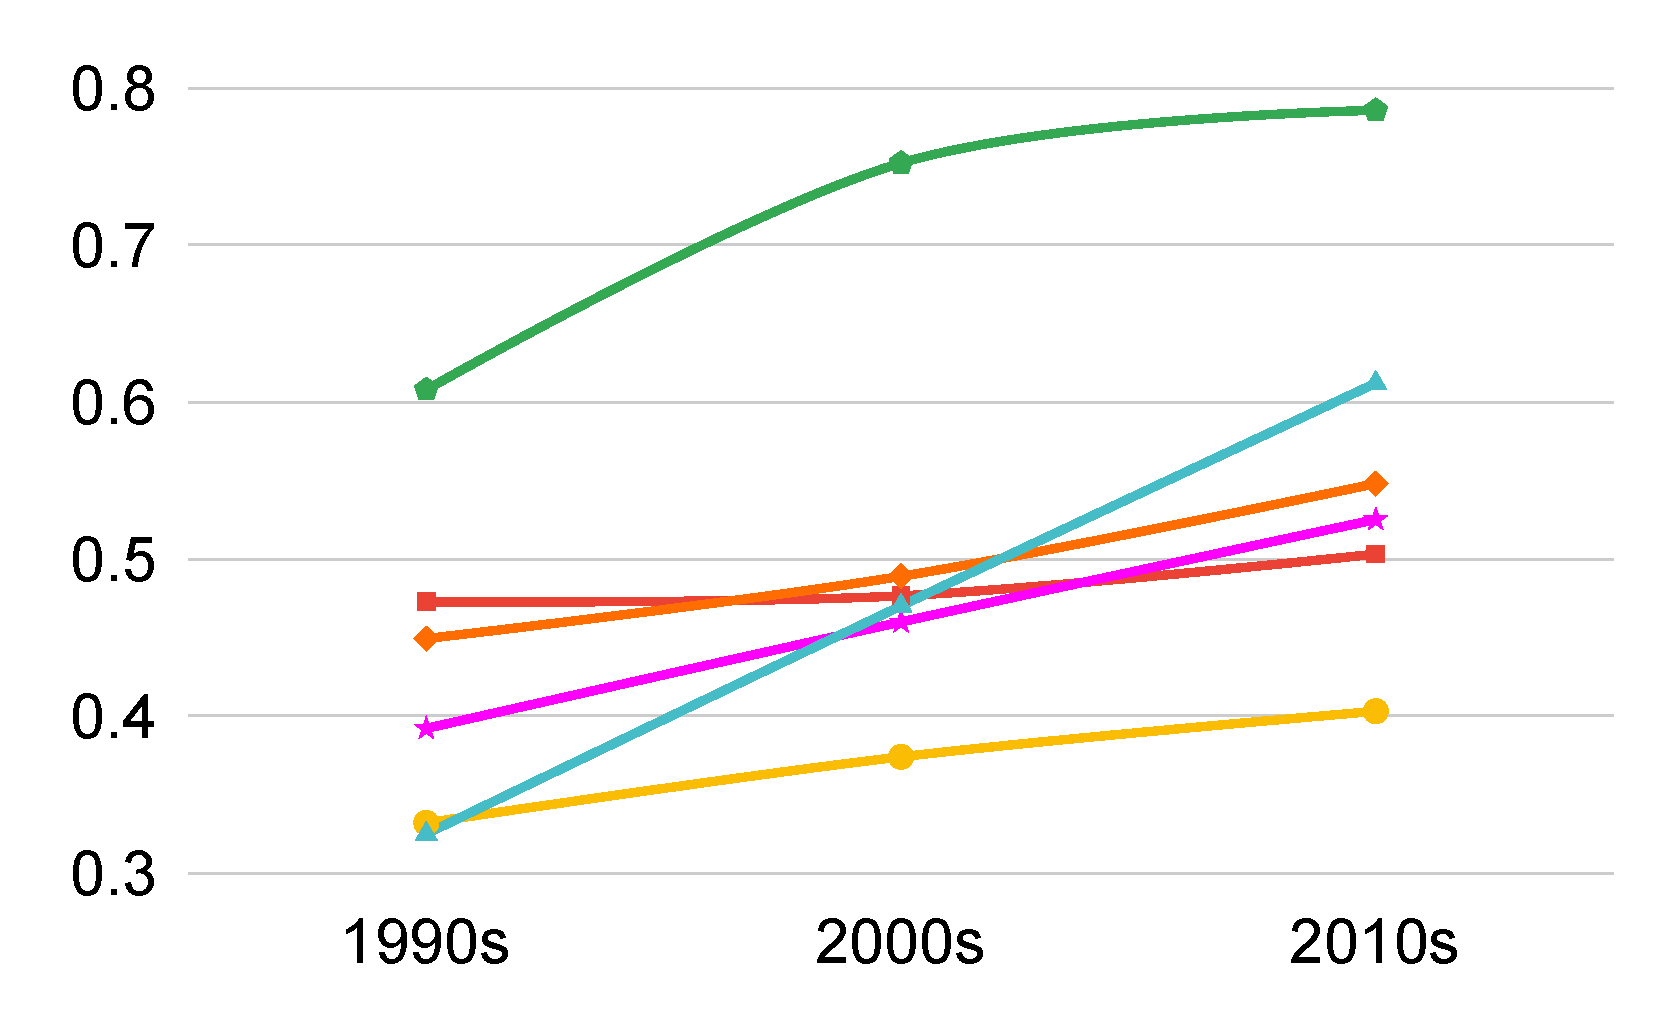
\includegraphics[width=\textwidth]{figures/VYLOMOVA_bullying-psych.pdf}
        \caption{Psychology}
  \end{subfigure}\begin{subfigure}[b]{.5\linewidth}
        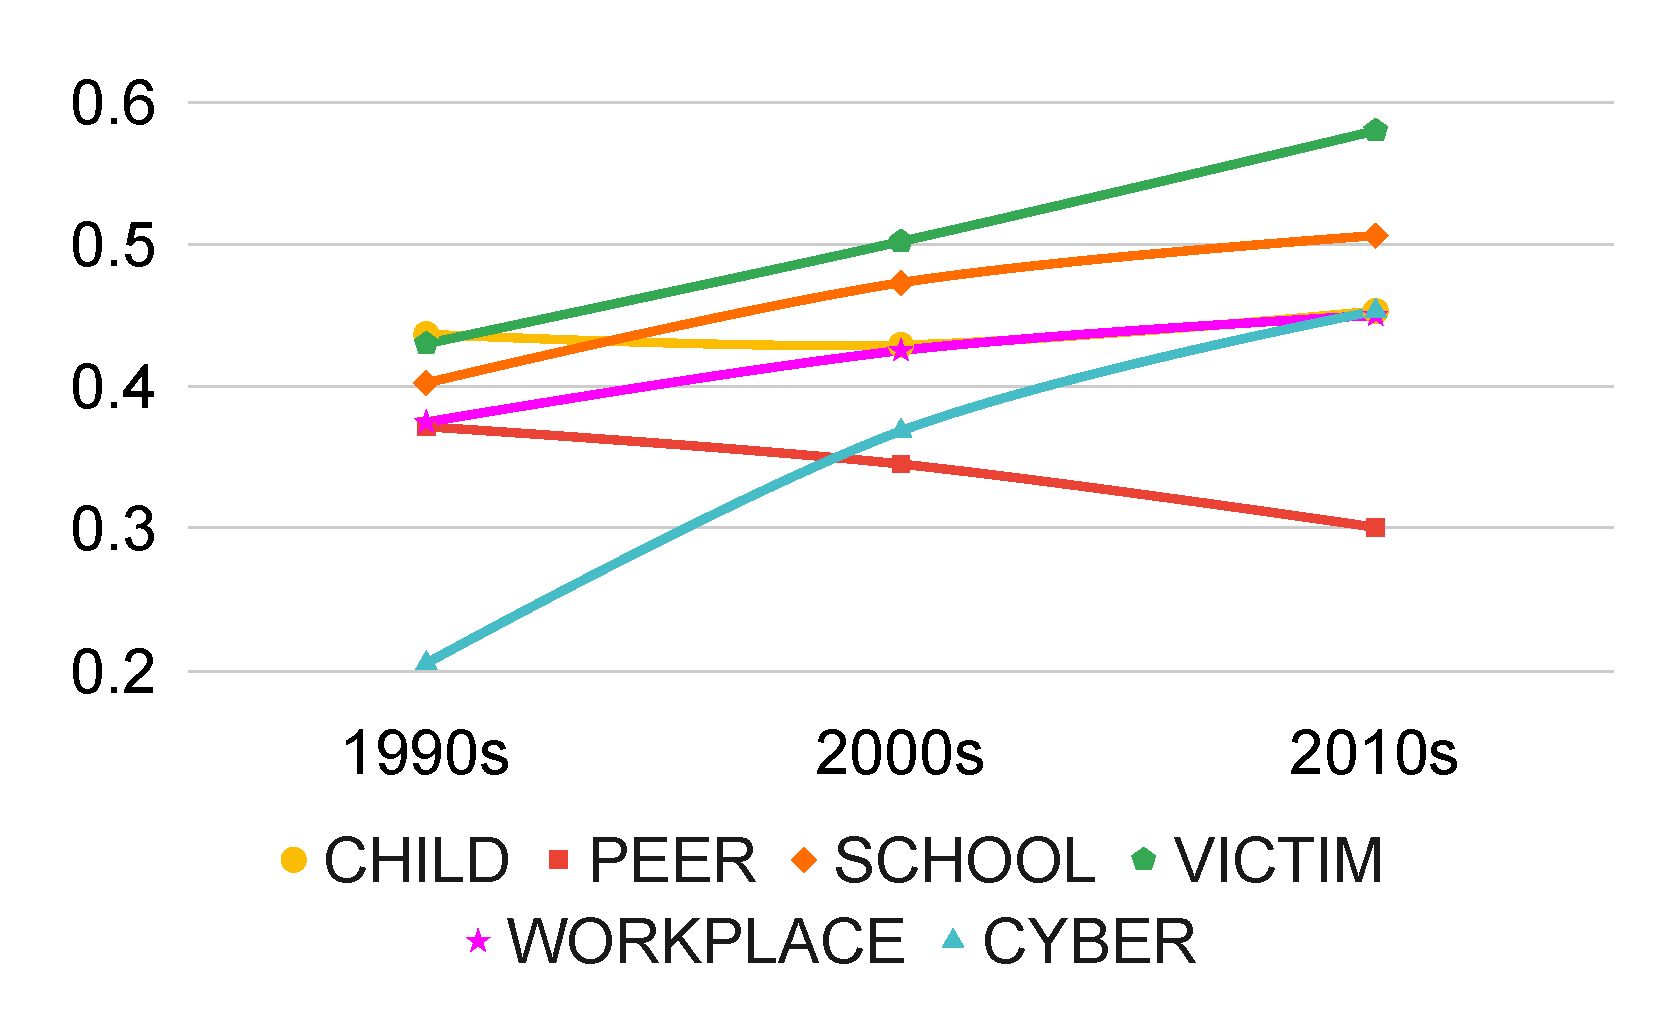
\includegraphics[width=\textwidth]{figures/VYLOMOVA_bullying-coca.pdf}
        \subcaption{General Domain (CoCA+CoHA)}
  \end{subfigure}
 \caption{`Bullying'. Cosine similarities over three decades\label{fig:w2v-cos-sim-bullying}}
\end{figure}

\begin{sloppypar}
In the psychology literature, `bullying' is also strongly intertwined with `harassment', and both are linked to the notion of \textit{victimization}. Arguably, this strong focus on victimization in the psychological literature, also evident in the concept of `harassment', represents a preoccupation with the harm caused by bullying. The results obtained on CoCA/CoHA appear to be less congruent and more noisy, and emphasize the behaviors involved in bullying rather than the harmful impact they have on their targets. Still, it is clear that `bullying' becomes more closely related to \textit{abuse} over time in that corpus but less related to \textit{aggression}.
\end{sloppypar}

\subsubsubsection{`Prejudice'}
In both corpora, but especially in psychology, `prejudice' is highly associated with \textit{racial} or \textit{racism}, both of which are also among its nearest neighbors during all decades (see Table~\ref{tab:prejudice-nns}). In the psychology corpus, the similarity is relatively stable while in CoCA/CoHA it reduces over time. The association of `prejudice' with \textit{ethnic} and \textit{ethnicity}, on the other hand, drops in both corpora. 
Dynamics of similarity with \textit{discrimination} presents differences: it decreases in CoCA/CoHA while it rises (along with similarity to \textit{anti-discrimination}) in psychology. The same pattern can be observed for \textit{gay}.
Interestingly, in the psychology corpus \textit{anti-gay} and \textit{pro-gay} are among the nearest neighbors and the similarity with \emph{both} of them increases over time, indicating a rising attention to anti-gay prejudice within psychology over time that is not seen in the general domain. This represents a ``horizontal'' expansion of `prejudice' in psychology beyond its earlier exclusive focus on racial animosity.\footnote{Among 200 nearest neighbors in each decade, the number of ``anti-'' and ``pro-'' terms is higher in psychology than in CoCA/CoHA.}  
Analysis of nearest neighbors shows that in both domains the associations between `prejudice' and \textit{stereotyping}, \textit{bigotry} and \textit{belief} are among the strongest and most stable over time.
In the psychology literature `prejudice' increases its similarity to \textit{micro-assault} and \textit{micro-insult} over the last decade. The growing relatedness to these forms of ``micro-aggression'' \citep{lilienfeld2017microaggressions} supports the claim that `prejudice' has crept ``vertically'' to encompass increasingly subtle phenomena. 

\begin{figure}
  \begin{subfigure}[b]{.5\linewidth}
        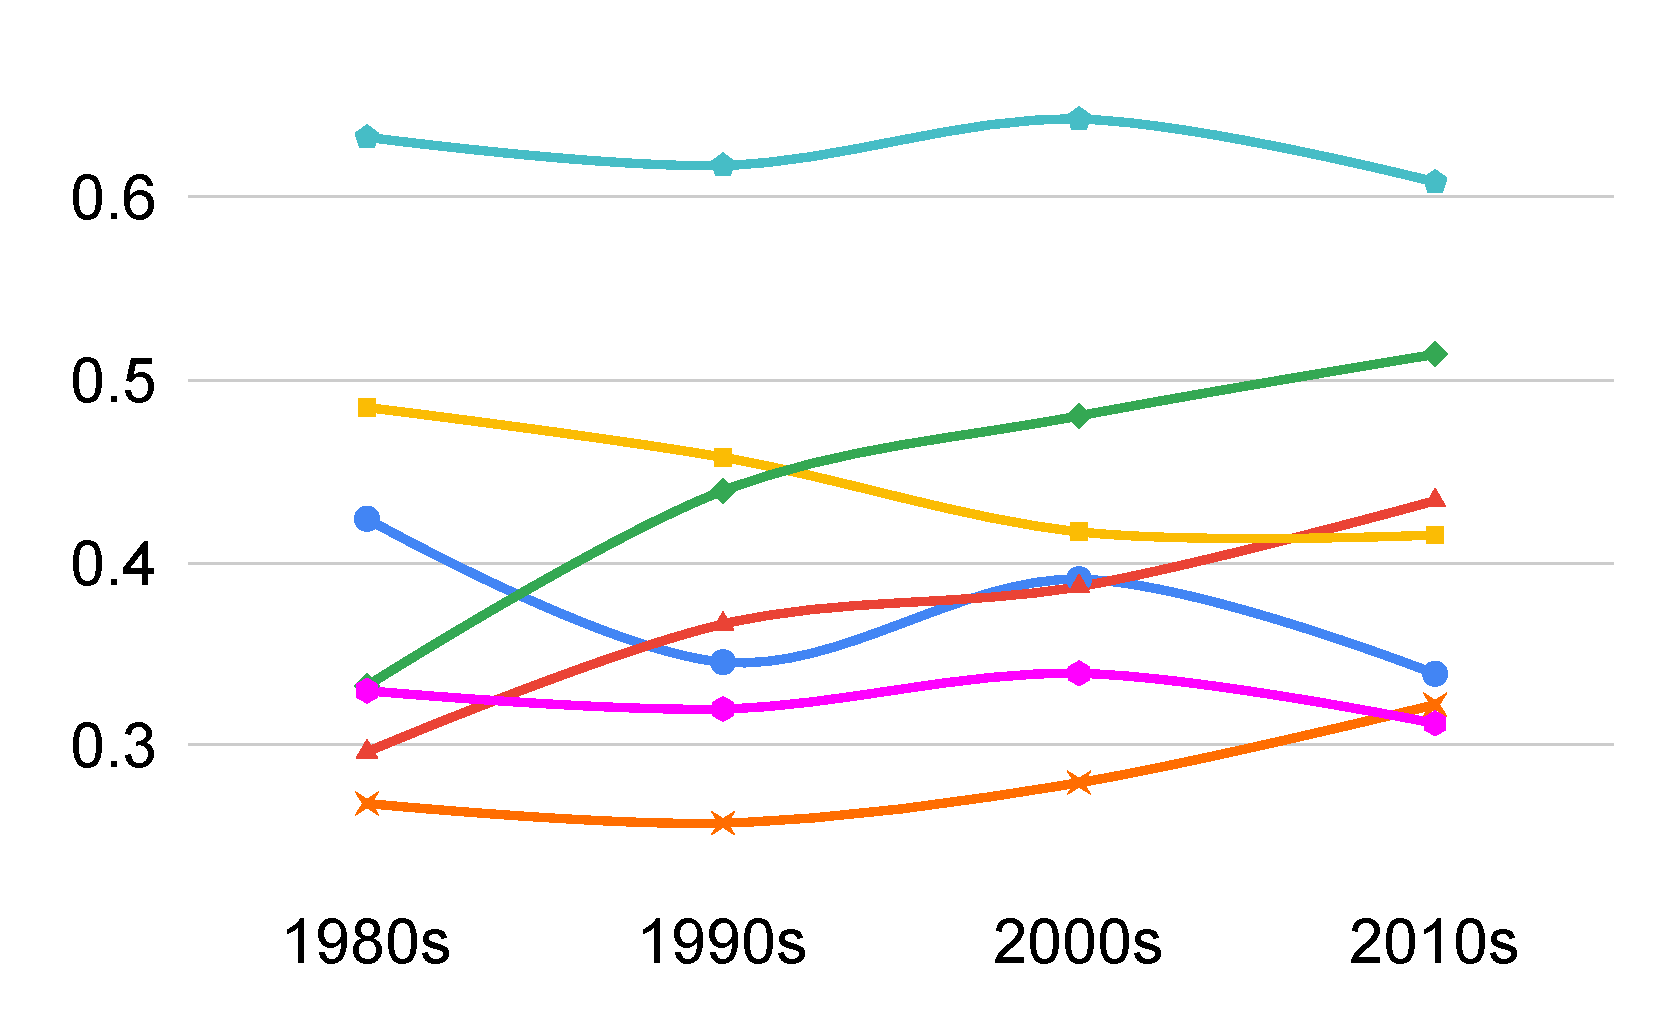
\includegraphics[width=.95\textwidth]{figures/VYLOMOVA_prejudice-psych.pdf}
        \caption{Psychology}
        \end{subfigure}\begin{subfigure}[b]{.5\linewidth}
        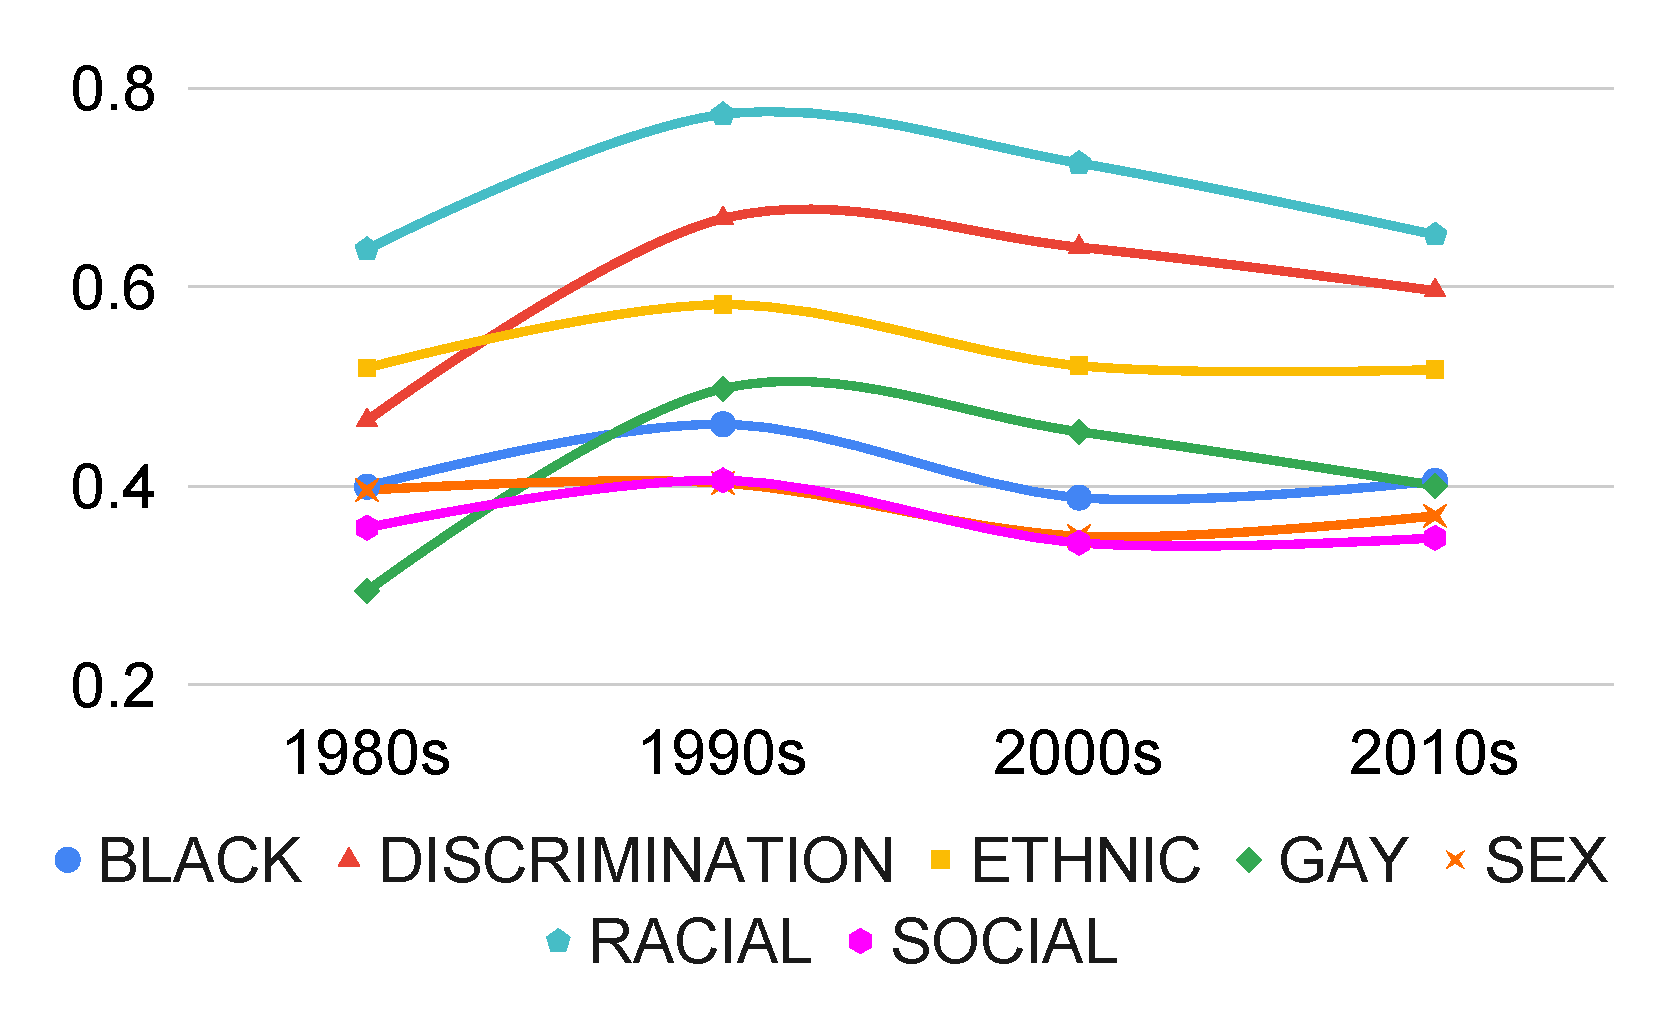
\includegraphics[width=\textwidth]{figures/VYLOMOVA_prejudice-coca.pdf}
        \caption{General Domain (CoCA+CoHA)}
        \end{subfigure}
 \caption{`Prejudice'. Cosine similarities over four decades.\label{fig:w2v-cos-sim-prejudice}}
\end{figure}

\begin{table}
\footnotesize
\caption{`Prejudice'. Top-10 nearest neighbors\label{tab:prejudice-nns}}
 \begin{tabular}{llll}
  \lsptoprule
\multicolumn{4}{c}{Psychology}\\
\multicolumn{1}{c}{1980s} & \multicolumn{1}{c}{1990s}  & \multicolumn{1}{c}{2000s} & \multicolumn{1}{c}{2010s}\\\midrule
prejudiced&prejudiced&prejudiced&prejudiced                   \\
ethnocentrism&antiblack&intergroup&intergroup                 \\
xenophobia&antiforeigner&stereotyping&blatant                 \\
racial&stereotyping&blatant&stereotyping                      \\
prejudicial&stereotype&outgroup&outgroup                      \\
racism&compunction&derogated&rwa                              \\
racist&prejudicial&sdo&sdo                                    \\
neuroessentialism&antigay&justif.suppression&authoritarianism \\
postcivil&racism&racism&derogated                             \\
ethnic&ethnopolitical&racist&antigay                          \\
ethnocentric&antifat&microinsult&justif.suppression           \\
justif.suppression&tropp&minoritygroup&homophobia             \\
sexblindness&antiatheist&majoritygroup&ideology               \\
sdo&antihomosexual&antigay&rightwing                          \\
transprejudice&justif.suppression&antihomosexual&minoritygroup\\
intelligentsia&oldfashioned&antiblack&microassault            \\
antiblack&neosexist&prejudicial&tropp                         \\
favoritism&intergroup&microinvalidation&antiforeigner         \\
microinsult&multiculturalist&ingroup&microinsult              \\
eugenics&problack&nonprejudicial&progay                       \\\midrule
\multicolumn{4}{c}{CoCA/CoHA}\\
\multicolumn{1}{c}{1980s} & \multicolumn{1}{c}{1990s}  & \multicolumn{1}{c}{2000s} & \multicolumn{1}{c}{2010s}\\\midrule
bigotry&racism&racism&bigotry\\
stereotyping&bias&bigotry&racism\\
racism&racial&racial&discrimination\\
racialist&bigotry&stereotype&stereotype\\
halfheartedness&discrimination&discrimination&racial\\
elitism&stereotype&injustice&ignorance\\
racial&prejudiced&racist&racist\\
belief&ignorance&colorism&belief\\
outsiderness&racist&hatred&oppression\\
uncomplicatedly&stereotyping&bias&bias\\
delegitimate&hatred&homophobia&classism\\
ridiculing&oppression&bigoted&misogyny\\
muddleheaded&injustice&belief&sexism\\
ethnocentrism&bigot&nonwhite&notion\\
factionalize&animosity&hostility&hatred\\
animus&homophobia&religion&discriminate\\
fact&bigoted&ignorance&denesh\\
biologism&sexism&speciesism&colorism\\
snideness&gender&semitism&prejudiced\\
multiculturalist&distrust&heterosexism&ridiculing\\
\lspbottomrule
\end{tabular}
\end{table}


\section{Conclusion}
 The findings of our analyses illuminate and add nuance to our understanding of concept creep within academic psychology and general domain corpora. The diachronic analysis reveals a trend for our sample of harm-related concepts to undergo semantic broadening from the 1970s to the 2010s, although the trajectories of particular concepts have been neither consistent nor linear. Since the 1990s, for example, `addiction', `bullying' and `harassment' have broadened, as the theory of concept creep would suggest, but the breadth of `trauma' and `prejudice' have been relatively static. The changes are more evident in psychology literature compared to CoCA/CoHA. The analysis of semantic displacement points to a more consistent diachronic pattern: the majority of concepts changed most substantially from the 1980s to the 1990s and changed progressively less thereafter. This finding implies that societal and cultural changes occurring in the final two decades of the 20th century are likely to be especially critical for understanding concept creep. Finally, the analysis of pairwise similarities demonstrated changing patterns of co-occurrence for each concept that clarified how its meanings have shifted and expanded over four decades. During this period some concepts have acquired entirely new associations (e.g., \textit{cyber-harassment}), some have added new semantic domains (e.g., `addiction' incorporating non-ingestive behaviors such as gaming and smartphone use), others have shifted emphasis (e.g., `trauma' becoming associated less with physical injury and more with psychological stress), and yet others have come to refer to less severe phenomena (e.g., `prejudice' becoming associated with so-called micro-aggressions). Collectively, these findings support the presence of both horizontal and vertical concept creep as proposed by \citet{haslam2016concept}.

The results of the present analyses are in some respects preliminary. From a methodological standpoint, future research will need to optimize the analytic parameters employed in the approaches examined in this research and evaluate whether findings derived from these approaches converge with those using other methods for assessing semantic change. Methods must also be developed to examine horizontal and vertical concept creep separately. The methods used in the present research emphasize ``horizontal'' changes in the range of semantic contexts in which a concept appears, and are less capable of capturing how meanings may shift ``vertically'' to encompass less severe phenomena. The latter can only be inferred indirectly when concepts referring to such subtler phenomena become increasingly near semantic neighbors of the target concept.

\begin{sloppypar}
Substantively, our findings should be replicated with additional hypothetically creeping concepts, such as `mental illness' and `safety'. The extent to which expansionary semantic changes are specific to harm-related concepts rather than generalized must also be studied systematically. There is scope for more focused and finely detailed analyses of semantic shifts in single concepts. Indeed, our approach offers a versatile methodology for evaluating the nature, timing, and nearest-neighbor subtleties of such shifts. Ideally, future work will explore concept creep in corpora representing other scholarly disciplines and other languages. A more fundamental challenge is to uncover the cultural factors that contribute to the semantic inflation of harm-related concepts, and to understand its societal implications.
\end{sloppypar}

\iffalse
\subsection{Emotion-based Analysis}
We then explore how the concepts changed in terms of basic emotions. For the purpose of the study, we utilize the list of basic emotions proposed in \citet{lazarus1994passion},\footnote{We excluded \emph{aesthetic experiences} from the list since it represents a more complex combination of emotions.} more specifically:
\begin{itemize}
    \item ``The nasty emotions'': \emph{anger} (anger, angry), \emph{envy} (envy), \emph{jealousy} (jealous*,jealousy)
    \item ``The existential emotions'': \emph{anxiety} (anxiety, anxious), \emph{fright} (fright*, frighten**), \emph{guilt} (guilt, guilty), \emph{shame} (shame, ashamed**,shameful**)
    \item ``Emotions provoked by unfavorable life conditions'': \emph{relief} (relief, relieve), \emph{hope} (hope), \emph{sadness} (sadness, sad), \emph{depression} (depression, depress)
    \item ``Emotions provoked by favorable life conditions'': \emph{happiness} (happy, happiness), \emph{pride} (pride*, proud**), \emph{love} (love)
    \item ``The empathetic emotions'': \emph{gratitude} (grateful**, gratitude*), \emph{compassion} (compassion**, compassionate**)
\end{itemize}


\begin{wrapfigure}{!h}{.6\textwidth}
        \centering
        {\includegraphics[width=.95\textwidth]{figures/VYLOMOVA_harassment-psych-emotions.pdf}
        \subcaption{Psychology}}\par\vfill
 \caption{\textbf{Harassment}. Cosine similarities to basic emotions.}
\label{fig:emotion-cos-sim-harassment}
\end{wrapfigure}


\begin{wrapfigure}{!h}{.6\textwidth}
        \centering
        {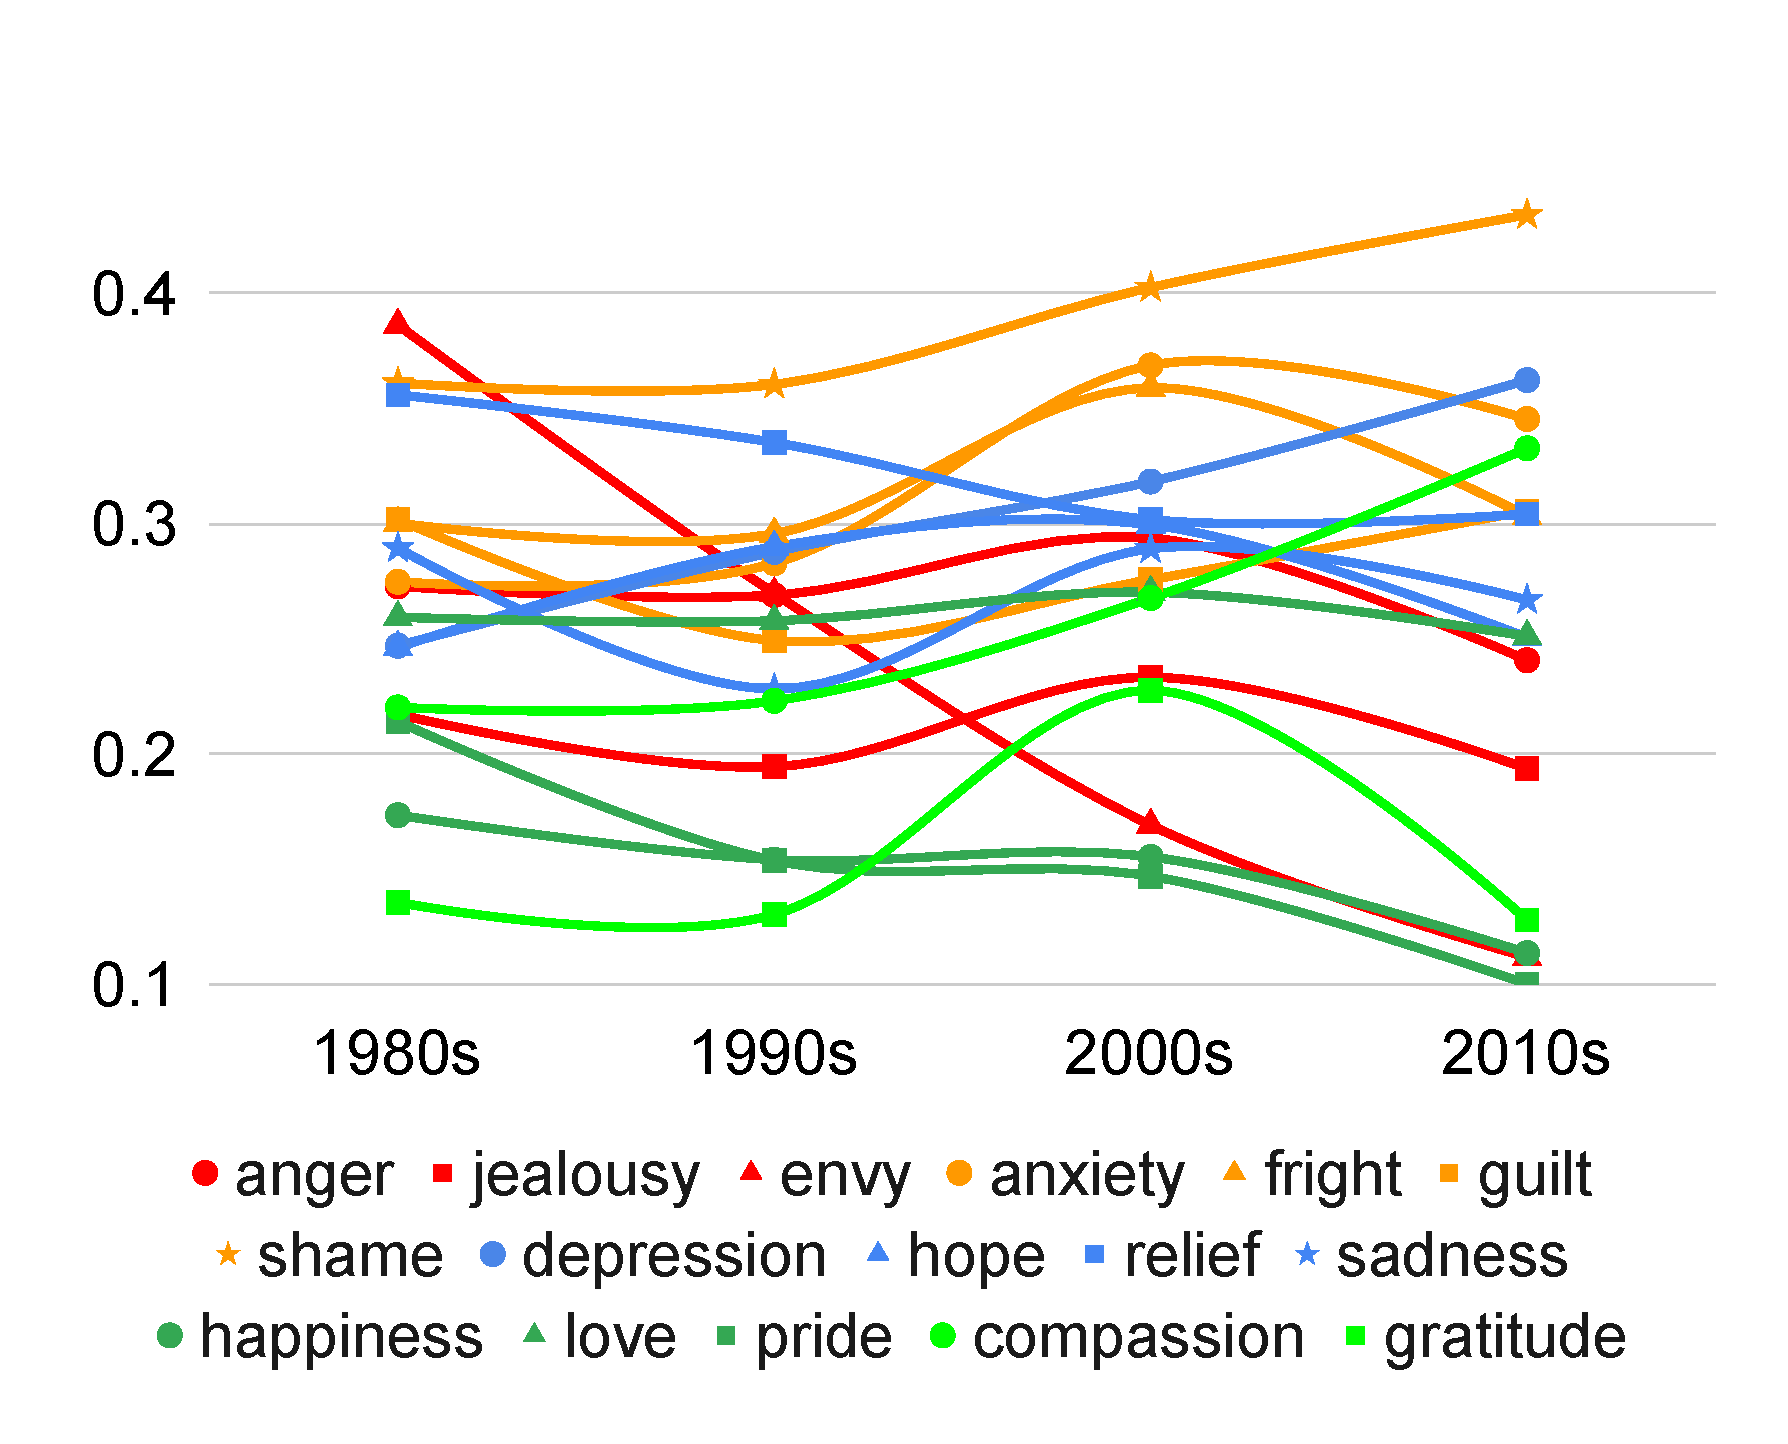
\includegraphics[width=.95\textwidth]{figures/VYLOMOVA_trauma-psych-emotions.pdf}
        \subcaption{Psychology}}\par\vfill
 \caption{\textbf{Trauma}. Cosine similarities to basic emotions.}
\label{fig:emotion-cos-sim-trauma}
\end{wrapfigure}



\begin{wrapfigure}{!h}{.6\textwidth}
        \centering
        {\includegraphics[width=.95\textwidth]{figures/VYLOMOVA_addiction-psych-emotions.pdf}
        \subcaption{Psychology}}\par\vfill
 \caption{\textbf{Addiction}. Cosine similarities to basic emotions.}
\label{fig:emotion-cos-sim-addiction}
\end{wrapfigure}

\begin{wrapfigure}{!h}{.6\textwidth}
        \centering
        {\includegraphics[width=.95\textwidth]{figures/VYLOMOVA_prejudice-psych-emotions.pdf}
        \subcaption{Psychology}}\par\vfill
 \caption{\textbf{Prejudice}. Cosine similarities to basic emotions.}
\label{fig:emotion-cos-sim-prejudice}
\end{wrapfigure}


\begin{wrapfigure}{!h}{.6\textwidth}
        \centering
        {\includegraphics[width=.95\textwidth]{figures/VYLOMOVA_bullying-psych-emotions.pdf}
        \subcaption{Psychology}}\par\vfill
 \caption{\textbf{Bullying}. Cosine similarities to basic emotions.}
\label{fig:emotion-cos-sim-bullying}
\end{wrapfigure}
\fi 

\section*{Abbreviations}
\begin{tabularx}{\textwidth}{@{}lQ@{}}
ACL & Association for Computational Linguistics\\
LSA & latent semantic analysis\\
PTSD & post-traumatic stress disorder\\
SVD & singular value decomposition\\
TF-IDF & term frequency - inverse document frequency \\
\end{tabularx}

{\sloppy\printbibliography[heading=subbibliography,notkeyword=this]}
\end{document}
